\documentclass[linenumbers,amsmath,trackchanges]{aastex702}
%%
%% \documentclass[argument1,argument2,argument3,...]{aastex7}
%%      Six of the arguments are typestting options. They are:
%%  twocolumn   : two text columns, 10 point font, single spaced article.
%%                This is the most compact and represent the final published
%%                derived PDF copy of the accepted manuscript from the publisher
%%  default     : one text column, 10 point font, single spaced (default).
%%  manuscript  : one text column, 12 point font, double spaced article.
%%  preprint    : one text column, 12 point font, single spaced article.  
%%  preprint2   : two text columns, 12 point font, single spaced article.
%%  modern      : a stylish, single text column, 12 point font, article with
%% 		  wider left and right margins. This uses the Daniel
%% 		  Foreman-Mackey and David Hogg design.
%% Note that you can submit to the AAS Journals in any of these 6 styles.
%%
%% There are other optional arguments one can invoke to allow other stylistic
%% actions. The available options are:
%%   linenumbers  : turn on linenumbering. Note this is mandatory for AAS
%%                  Journal submissions and revisions.
%%   trackchanges : Shows added text in bold.
%%   longauthor   : Do not use the more compressed footnote style (default) for 
%%                  the author/collaboration/affiliations. Instead print all
%%                  affiliation information after each name. Creates a much 
%%                  longer author list but may be desirable for short 
%%                  author papers.
%% twocolappendix : make 2 column appendix.
%%   anonymous    : Do not show the authors, affiliations, acknowledgments,
%%                  and author contributions for dual anonymous review.
%%  resetfootnote : Reset footnotes to 1 in the body of the manuscript.
%%                  Useful when there are a lot of authors and affiliations
%%		    in the front matter.
%% Since v6, AASTeX has included \hyperref support. While we have built in 
%% specific %% defaults into the classfile you can manually override them 
%% with the \hypersetup command. For example,
%% \hypersetup{linkcolor=red,citecolor=green,filecolor=cyan,urlcolor=magenta}
%% will change the color of the internal links to red, the links to the
%% bibliography to green, the file links to cyan, and the external links to
%% magenta. Additional information on \hyperref options can be found here:
%% https://www.tug.org/applications/hyperref/manual.html#x1-40003


\usepackage[margin=1in]{geometry}
\usepackage{graphicx}
\usepackage{xcolor}
\usepackage{amsmath}
 
\graphicspath{{figures/}}


%% If you want to create your own macros, you can do so
%% using \newcommand. Your macros should appear before
%% the \begin{document} command.
%%
\newcommand{\vdag}{(v)^\dagger}
\newcommand\aastex{AAS\TeX}
\newcommand\latex{La\TeX}
%%%%%%%%%%%%%%%%%%%%%%%%%%%%%%%%%%%%%%%%%%%%%%%%%%%%%%%%%%%%%%%%%%%%%%%%%%%%%%%%
%%
%% The following section outlines numerous optional output that
%% can be displayed in the front matter or as running meta-data.
%%
%% Running header information. A short title on odd pages and 
%% short author list on even pages. Note that this
%% information may be modified in production.
%%\shorttitle{AASTeX v7.0.2 Sample article}
%%\shortauthors{The Terra Mater collaboration}
%%
%% Include dates for submitted, revised, and accepted.
%%\received{February 1, 2025}
%%\revised{March 1, 2025}
%%\accepted{\today}
%%
%% Indicate AAS Journal the manuscript was submitted to.
%%\submitjournal{PSJ}
%% Note that this command adds "Submitted to " the argument.
%%
%% You can add a light gray and diagonal water-mark to the first page 
%% with this command:
% \watermark{DRAFT}
 
\begin{document}  
 
\title{Improved Probabilistic Star-Galaxy Separation Method for Rubin LSST Catalogs}
 
\correspondingauthor{{\v Z}eljko Ivezi{\'c}}
 
\author[0000-0001-5250-2633, gname=\v{Z}eljko, sname=Ivezi\'{c}]{\v{Z}eljko Ivezi\'{c}}
\affiliation{Department of Astronomy, University of Washington, Box 351580, Seattle, WA 98195, USA}
\email[show]{ivezic@uw.edu}

\author[0009-0004-0944-9098]{Jinshuo Zhang} 
\affiliation{Department of Astronomy, University of Washington, Box 351580, Seattle, WA 98195, USA}
\email{jinshuoz@uw.edu} 

\author{Nirav Nemali}
\affiliation{Department of Astronomy, University of Washington, Box 351580, Seattle, WA 98195, USA}
\email{niravn6@uw.edu}

\author{Dan Taranu}
\affiliation{Department of Astrophysical Sciences, Princeton University, Princeton, NJ 08544, USA}
\email{dan.s.taranu@gmail.com}  

\author{Colin T. Slater}
\affiliation{Department of Astronomy, University of Washington, Box 351580, Seattle, WA 98195, USA}
\email{ctslater@uw.edu} 

\author{Robert H. Lupton}
\affiliation{Department of Astrophysical Sciences, Princeton University, Princeton, NJ 08544, USA}
\email{rhl@astro.princeton.edu} 

\author{other Rubin coauthors}
\affiliation{Rubin Observatory}
\email{verarubin@noirlab.edu} 



\begin{abstract}
The morphological classification of resolved and unresolved sources, commonly referred to as ``star-galaxy
separation'', is a fundamental step in the analysis of wide-field imaging surveys such as Rubin Observatory's
Legacy Survey of Space and Time (LSST). Star-galaxy separation becomes increasingly challenging at
the faint magnitudes
probed by LSST because galaxy counts rise rapidly  with magnitude while their angular sizes become
progressively smaller. LSST photometric catalogs provide a binary classifier \texttt{extendedness} in each band, based on the
threshold difference between PSF, \(m_{\mathrm{PSF}}\), and CModel, \(m_{\mathrm{CModel}}\),
magnitudes.  While this parameter provides a useful baseline for morphological classification, its binary nature
prevents the optimal combination of information from multiple bands, as well as from other
classification methods (e.g., those based on colors or external datasets). In this work, we implement
the Bayesian star-galaxy classification method of Slater, Ivezi\'{c} \& Lupton (2020), which overcomes these shortcomings.
In each band, we model the distribution of sources in the two-dimensional space defined by
\(\Delta m = m_{\mathrm{PSF}} - m_{\mathrm{CModel}}\) and magnitude \(m_{\mathrm{CModel}}\).
At a fixed magnitude, the distribution is modeled as a mixture of unresolved and resolved
components which, with appropriately chosen priors for the star-to-galaxy number ratio, allows us to
compute \(p_S\), the posterior probability that a source is unresolved.
We apply this method to the Rubin Data Preview 2 object catalog and validate the resulting classifications using external HST
labels in the COSMOS field. Using these labels as the ground truth, we quantitatively compare the performance of the \(p_S\)-based
classifier with that of the Rubin \texttt{extendedness} parameter. We find that the \(p_S\)-based classifier
consistently outperforms the Rubin \texttt{extendedness} baseline, with the improvement
increasing as additional bands are incorporated.  Approximately, the \(p_S\) classifier
achieves the same classification performance at a magnitude limit about half a 
magnitude fainter than the \texttt{extendedness} classifer. Depending on the scientific
application, this morphological classification can be further improved by incorporating
complementary color-based classifiers.
\end{abstract}

%% Keywords should appear after the \end{abstract} command. 
%% The AAS Journals now uses Unified Astronomy Thesaurus (UAT) concepts:
%% https://astrothesaurus.org
%% You will be asked to selected these concepts during the submission process
%% but this old "keyword" functionality is maintained in case authors want
%% to include these concepts in their preprints.
\keywords{\uat{Galaxies}{573} --- \uat{Cosmology}{343}  --- \uat{Stellar astronomy}{1583} --- \uat{Solar physics}{1476}}

\date{\today}

%\input{methodSummary}


55\section{Introduction}

The morphological classification of resolved and unresolved sources\footnote{Note that some stars can be
resolved, such as Asymptotic Giant Branch stars, while quasars and galaxies can be unresolved.}, commonly
referred to as ``star-galaxy separation'', is a fundamental step in the analysis of wide-field imaging surveys
such as the Rubin's Legacy Survey of Space and Time (LSST). At bright magnitudes this problem is
relatively simple, since stars outnumber galaxies and the galaxies that do exist are obviously extended on the sky.
Star-galaxy separation becomes increasingly harder at faint magnitudes, such as those probed by
Rubin's Legacy Survey of Space and Time (LSST; for details see \citealt{2019ApJ...873..111I} and references therein)
because galaxy counts rapidly increase with magnitude, while their angular sizes become smaller.

A variety of methods have been proposed in the literature for morphological classification of sources in images. 
\cite{2020AJ....159...65S} (hereafter SIL2020) discussed the statistical foundations of morphological star–galaxy separation and showed
that many of the star-galaxy separation metrics in common use today, e.g., by Sloan Digital Sky Survey (SDSS) {\it photo}
pipeline \citep{2002SPIE.4836..350L}, or SExtractor pipeline \citep{1996A&AS..117..393B}, are closely
related both to each other, and to the Bayesian model odds ratio, first derived by \cite{1979AJ.....84.1526S}.
SIL2020 quantified the scaling of various algorithms with the source noise properties and showed that the Bayesian model
odds ratio achieves the best peformance. They also showed how to probabilistically combine multiple measurements,
either of the same type (e.g., subsequent exposures), or differing types (e.g., multiple bandpasses), or differing
methodologies (e.g., morphological and color-based classification).

Following SDSS, LSST photometric catalogs use a binary classifier \texttt{extendedness} in each band, based on the
threshold difference between PSF, \(m_{\mathrm{PSF}}\), and CModel, \(m_{\mathrm{CModel}}\),
magnitudes, \(\Delta m = m_{\mathrm{PSF}} - m_{\mathrm{CModel}}\). For unresolved sources, this \(\Delta m \)
is vanishing within noise, with \texttt{extendedness=0}, while for resolved objects, selected by \(\Delta m >
0.016\) mag, \texttt{extendedness=1}. Resolved objects have positive \(\Delta m \) because their
PSF flux is smaller than CModel flux due to a narrow weighting PSF profile. For an illustration of \(\Delta m \)
distribution in Rubin's Data Preview 1 catalogs, see Fig.~28 in \cite{2026AJ....171..360V}. 

Although  \texttt{extendedness} was successfuly used in thousands of papers based on SDSS catalogs, this
approach is not optimal for LSST. As discussed in SIL2020, when the star-galaxy separation threshold is optimized
at the faint, low S/N, end of the data, the ability to recognize barely resolved objects at the bright end is not fully exploited. 
More importantly, the binary nature of \texttt{extendedness} parameter prevents optimal combination of information from
different bands, as well as from other classification methods (e.g., based on colors, or other datasets). SIL2020 showed how
to turn \(\Delta m \) into a probability distribution, which then allows proper probabilistic combination of multiple bands.
With appropriately chosen priors for star-to-galaxy counts ratio, the posterior probability that a source is unresolved
(or resolved), can be computed in Bayesian framwork. 

The main goal of this paper is to implement the steps towards Bayesian star-galaxy separation outlined in SIL2020
using Rubin's Data Preview 2 data. We describe our dataset and method in \S 2, and quantify its performance using
HST-based labels in \S 3. We discuss our results and how to retrieve our catalog with improved star-galaxy separation in \S 4. 
 

\providecommand{\FloatBarrier}{\clearpage}
\renewcommand{\topfraction}{0.92}
\renewcommand{\bottomfraction}{0.85}
\renewcommand{\textfraction}{0.06}
\renewcommand{\floatpagefraction}{0.75}
\setcounter{topnumber}{3}
\setcounter{bottomnumber}{2}
\setcounter{totalnumber}{5}


\section{Datasets}
\label{sec:data-methods}

Here we describe two principal datasets used in our analysis: Rubin Data Preview 2 catalogs and HST
data with star-galaxy labels used for testing methods discussed in \S 3. 


\subsection{Rubin Data Preview 2} 
\label{sec:data}

All data collected with the LSST Camera \cite{RTN-115} during the commissioning of the Rubin Observatory
will be released as Data Preview 2\footnote{See https://dp2.lsst.io/} (hereafter DP2). Coadded deep images and resulting catalogs have
been released in July 2026 as Early Data Preview 2. These coadded images are based on about 24,000
single-visit images and cover about 3,000 sq. deg. of sky. 

In our analysis we focus on the COSMOS field because it is both already well observed by Rubin (to
only about 1 magnitude shallower limit than anticipated for 10-year LSST), and space-based HST
COSMOS2020/FARMER star and galaxy labels are available \citep{2022ApJS..258...11W}. As a control
sample for testing code robustness, we also used Rubin data for the Extended Chandra Deep Field South (ECDFS). 
The Rubin $5-\sigma$ depth for point sources in the COSMOS field, estimated as the median magnitude
of point sources with photometric errors of $\sim$0.2 mag, is (25.66, 26.66, 26.36, 25.91, 24.94, 23.59)
in the $ugrizy$ bands, respectively. 


\subsection{HST Star-galaxy Classification Labels in the COSMOS Field} 

For the COSMOS validation sample, we select Rubin DP2 sources in the rectangular region
\(149.7 < {\rm RA} < 150.7\) and \(1.7 < {\rm Dec} < 2.7\), with
\(16 \le r_{\rm CModel} < 26\). Objects listed in the COSMOS2020/FARMER reference catalog are
matched to DP2 sources using a 0.5 arcsec matching radius. Within the selected region and magnitude
ranges, the DP2 sample contains 269,606 objects, of which 193,586 are matched to the
COSMOS2020/FARMER objects and 76,020 are unmatched (a matching fraction of 72\%). This
somewhat low matching fraction is due to large areas around bright stars that are masked in the
COSMOS2020/FARMER catalog (see Figure~\ref{fig:cosmos-footprint}). 

The matched validation sample contains 8,788 stars and 184,798 galaxies, classified using
HST's \(\texttt{truth\_binary}=1\) for stars and \(\texttt{truth\_binary}=0\) for galaxies. Their number
counts as function of magnitude are shown in Figure~\ref{fig:cosmos-magnitude-distribution}.
The low fraction stars is due to very faint sample limit $r \sim 26$) and high Galactic latitude ($b \sim
50^\circ$).  

\begin{figure*}[t]
  \centering
  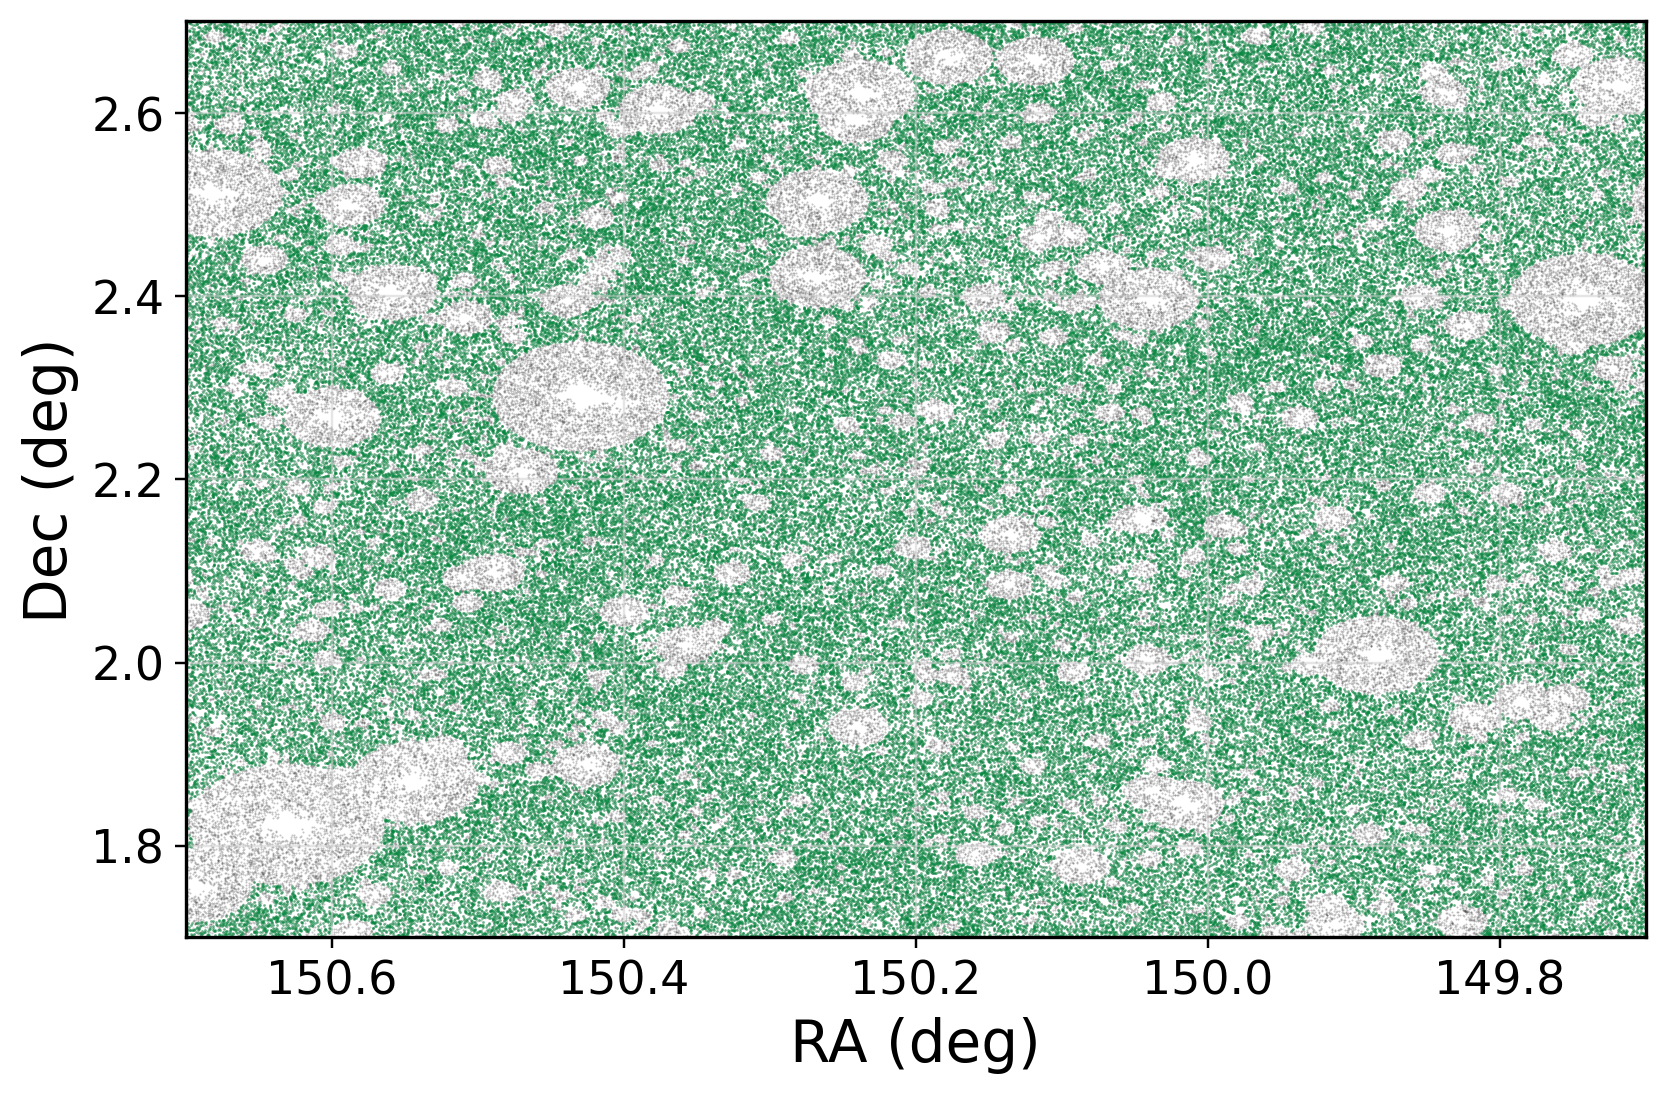
\includegraphics[width=0.9\textwidth]{fig01_cosmos_sky_coverage.png}
  \caption{
  The footprint for the DP2-COSMOS sample analyzed here. Gray points show Rubin DP2 objects 
  and  green points show the subset matched to the HST COSMOS2020/FARMER sample  
  a 0.5 arcsec matching radius. The white regions in the centers of gray areas correspond to
  areas where no objects are listed in either catalog. 
  }
  \label{fig:cosmos-footprint}
\end{figure*}

\begin{figure*}[t]
  \centering
  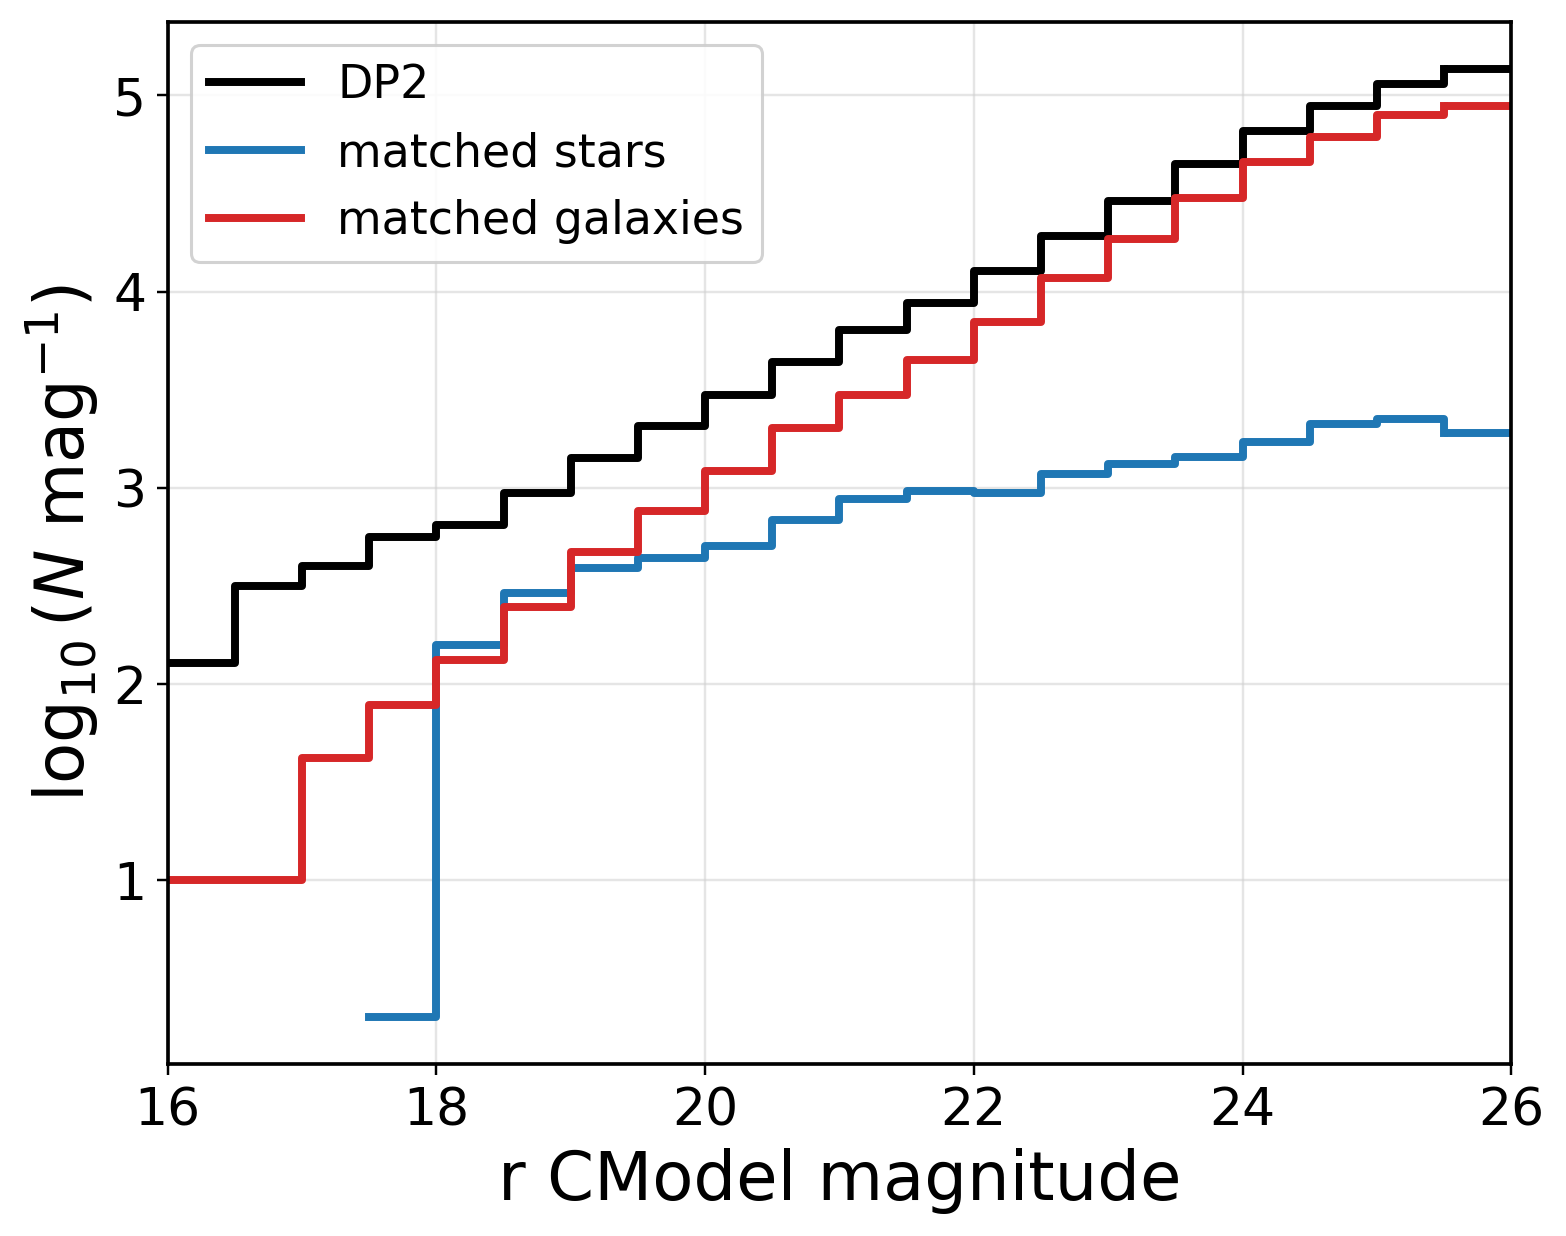
\includegraphics[width=0.8\textwidth]{fig02_cosmos_dataset_overview.png}
  \caption{
  Magnitude distribution of the DP2-COSMOS sample. The black curve shows
  all selected DP2 sources, while the blue and red curves show matched
  COSMOS2020/FARMER sources classified as stars and galaxies, respectively.
  Counts are shown per magnitude, using 0.5 mag wide bins.  Note that galaxies
  outnumber stars at the faint end by more than an order of magnitude. 
  }
  \label{fig:cosmos-magnitude-distribution}
\end{figure*}



\subsection{The color-magnitude distributions of sources classified using HST labels}
\label{sec:reference-distributions}

The external COSMOS2020/FARMER labels provide the reference classification, considered here as ground
truth, for examining the distribution of stars and galaxies in various diagrams and for measuring
the performance of star-galaxy separation methods. Nevertheless, it is likely that some very faint
sources classified by HST as stars might be unresolved galaxies even at HST's resolution. Therefore,
the HST labels will help us assess whether a source should be resolved or unresolved in Rubin
images, but do not necessarily provide definitive information about astrophysical nature of a source
(e.g., to separate unresolved stars and galaxies, one would need spectra or broad-band photometry
over a much wider weavelength range, say, in near-infrared $K$ band). Furthermore, no classification
is perfect and thus we first examine the distribution of HST-classified ``stars`` and ``galaxies`` in
various informative color-color diagrams constructed with Rubin photometry. 

The top left panel in Figure~\ref{fig:truth_morphology_color} shows the distribution of stars and galaxies classified
using HST labels in the \(\Delta m = m_{\mathrm{PSF}} - m_{\mathrm{CModel}}\) vs. \(m_{\mathrm{CModel}}\)
diagram. As we describe in detail in the next Section, modeling this distribution is a key ingredient of the
Bayesian star-galaxy separation method presented here. 


The top right panel in Figure~\ref{fig:truth_morphology_color} shows that faint galaxies ($r>24$),
in addition to outnumbering stars at faint magnitudes, have on average bluer $g-i$ colors than stars. 
The clearly different distributions of stars and galaxies in color-color diagrams shown in the bottom
two panels in Figure~\ref{fig:truth_morphology_color}
demonstrate that colors can be used to enhance morphological star-galaxy separation. 
Nevertheless, Figure~\ref{fig:truth_color_color} and the top left panel in
Figure~\ref{fig:truth_morphology_color} clearly show that increased photometric noise close to the faint
magnitude limit will cause deteriorated performance for both morphological and color-based
star-galaxy separation methods. Extending the start of this deterioration to a fainter magnitude
limit is one of the primary goals of this work.  It is notable that the top right panel in Figure~\ref{fig:truth_color_color} 
implies that most unresolved faint blue sources have $u-g$ color more typical of low-redshift
quasars than of main sequence stars (for a detailed discussion of the blue star counts see
\citealt{2026A&A...707A.333P}). 


\begin{figure*}
  \centering
  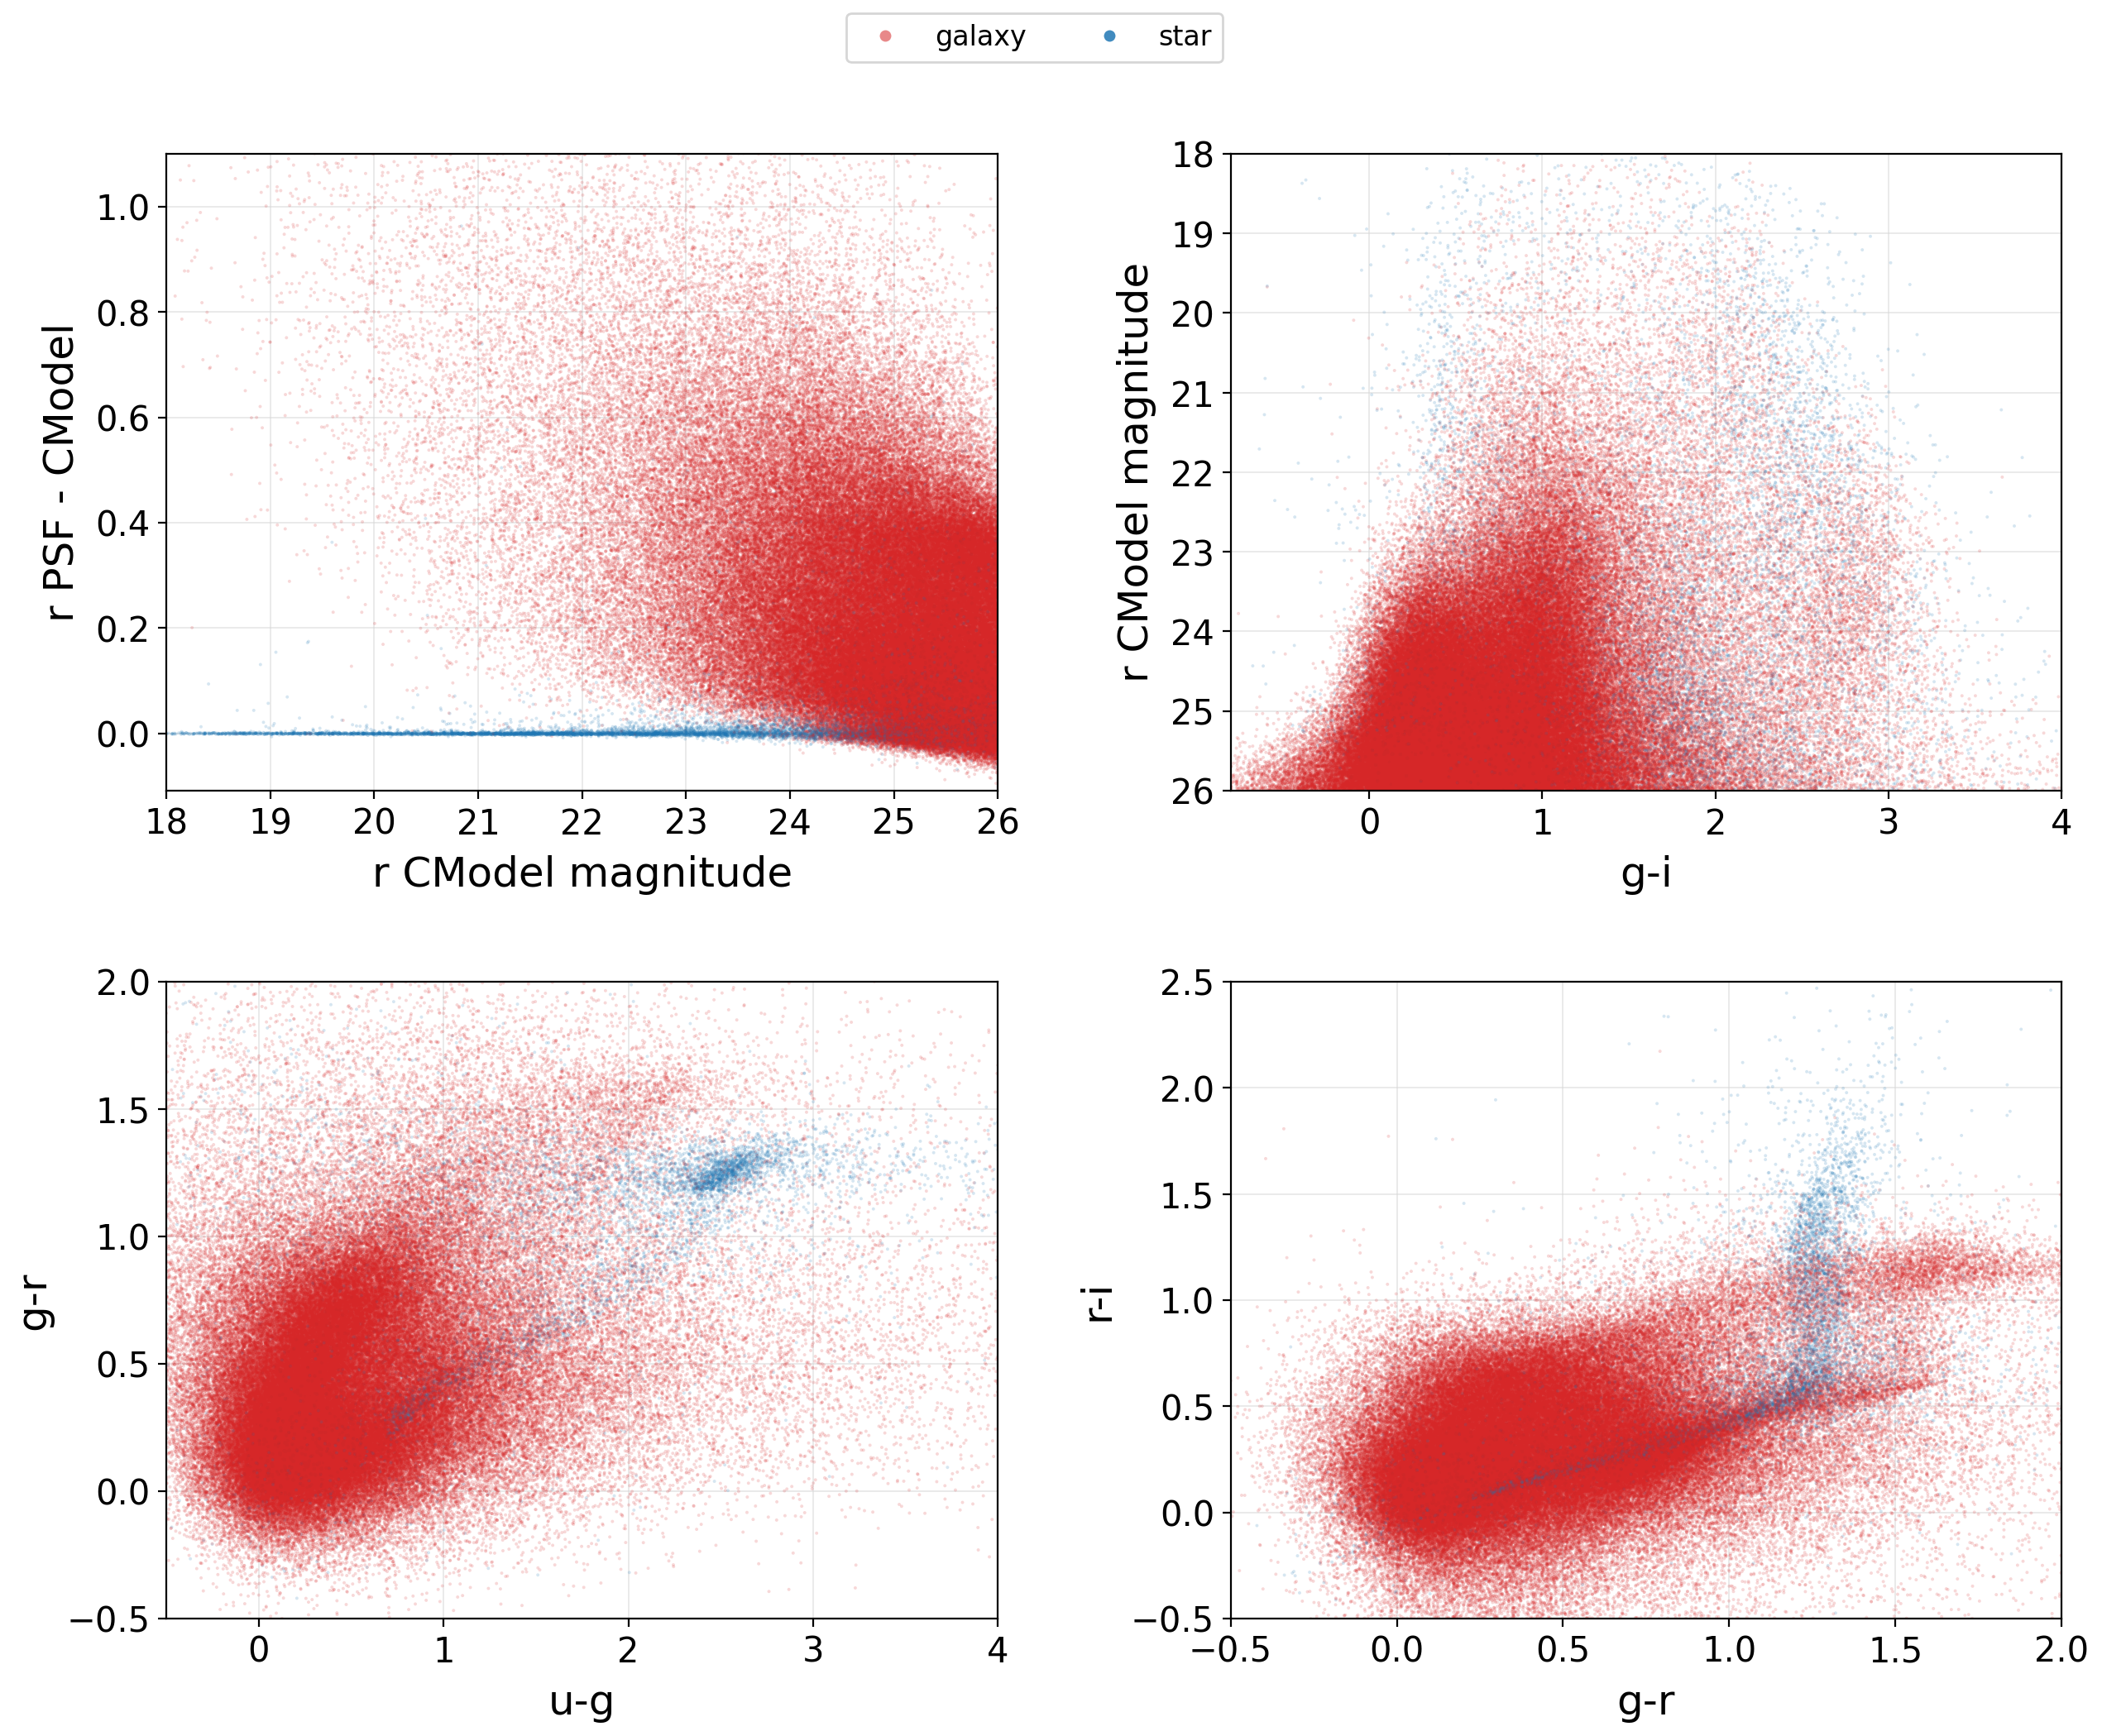
\includegraphics[width=\textwidth]{fig03_truth_morphology_color.png}
  \caption{The distribution of stars (blue dots) and galaxies (red countours), classified using HST labels, in various infomative
    diagrams. The CModel-magnitude based colors are corrected for the ISM dust extinction, while the $r$-band CModel magnitude is not.
   The top left panel shows the \(\Delta m = m_{\mathrm{PSF}} - m_{\mathrm{CModel}}\) vs. \(m_{\mathrm{CModel}}\) diagram, where
   stars form a narrow sequence centered on \(\Delta m \approx 0\) and for galaxies \(\Delta m >  0 \).  
   The top right panel shows the $r$ vs. $g-i$ color magnitude diagram and two bottom panels show
   most informative color-color diagrams. The main stellar locus, dominated by main sequence stars
   and red giants, is clearly visible with its blue end redwards from $u-g \sim 0.6$; unresolved sources with $u-g < 0.6$ are expected to be a
   mixture of low-redshift quasars, white dwarfs and unresolved binaries.}
  \label{fig:truth_morphology_color}
\end{figure*}


\begin{figure*}
  \centering
  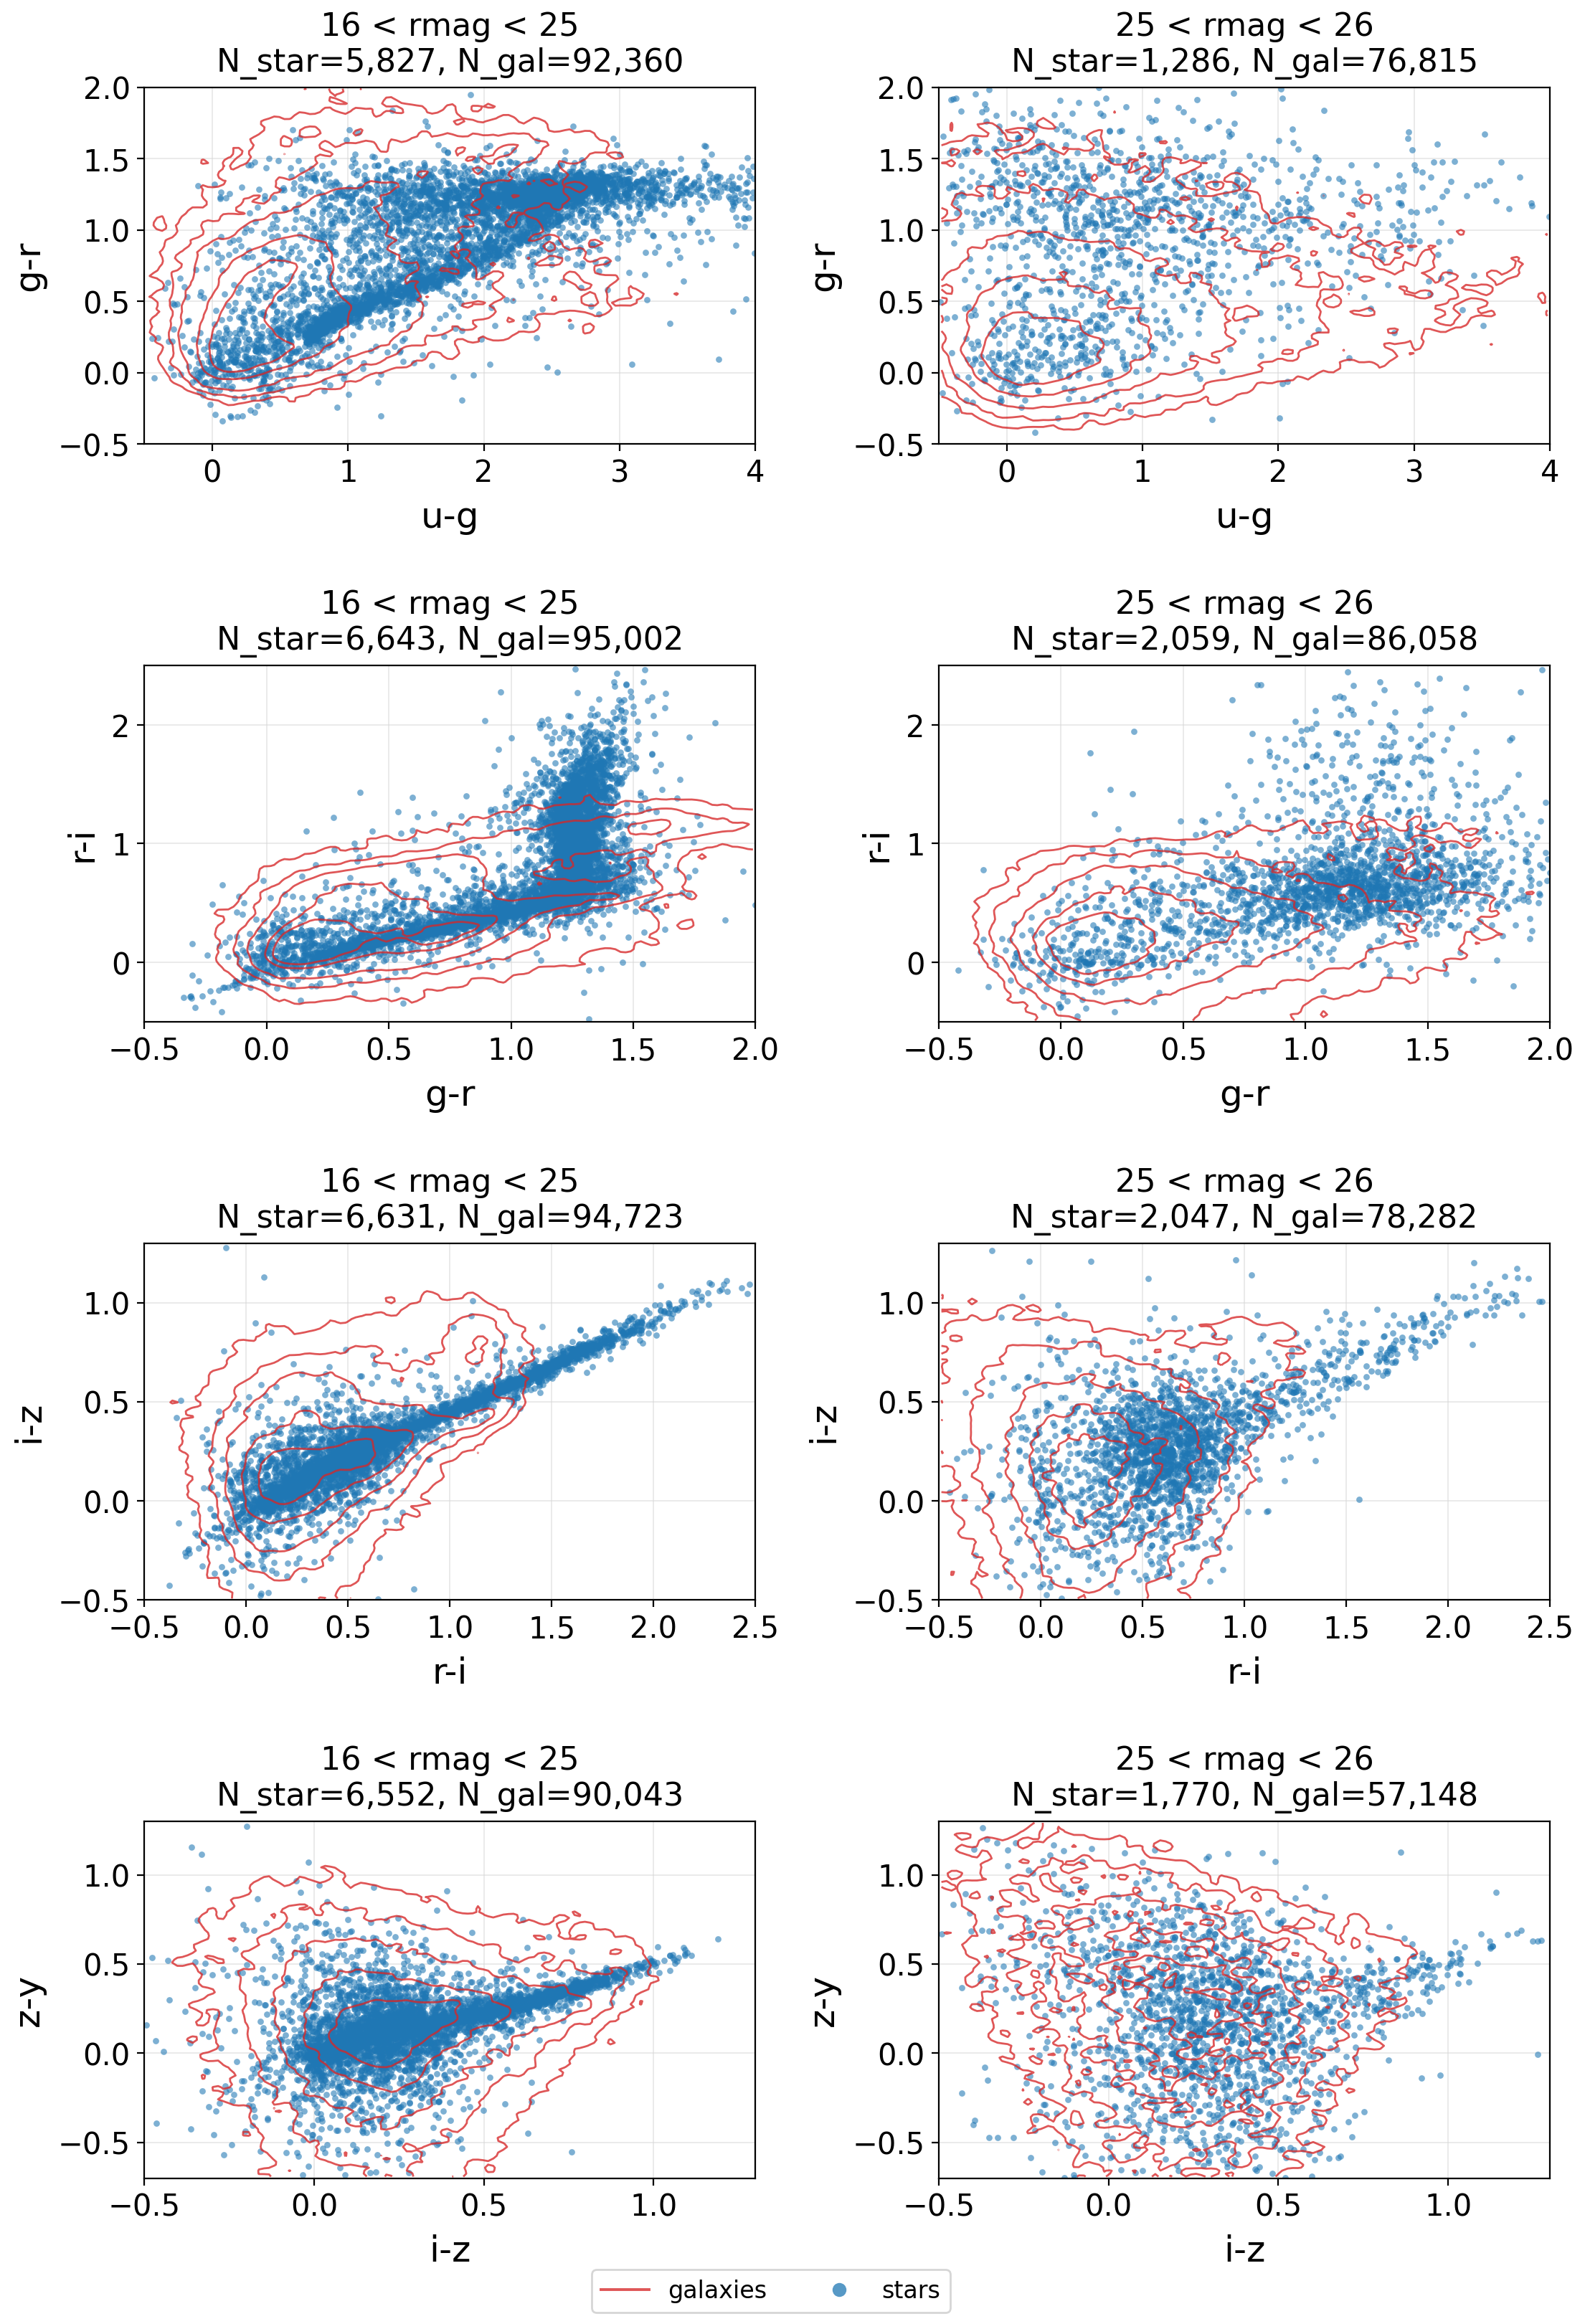
\includegraphics[width=0.8\textwidth]{fig04_truth_color_color.png}
  \caption{Similar to the bottom two panels in Figure~\ref{fig:truth_morphology_color}, except that
   here all principal color-color diagrams are shown and the data are split by the $r$-band CModel magnitude
   to show deterioration of photometry close to the faint magnitude limit (left: 16 $<$ rmag $<$ 25; right: 25 $<$
   rmag $<$ 26). The $5-\sigma$ depth for point sources in the $r$ band for this dataset is 26.36.}
  \label{fig:truth_color_color}
\end{figure*}

 

\subsection{The color-magnitude distributions of sources classified using \texttt{extendedness} parameter} 
\label{sec:extendedness-baseline}

Difficulties with star-galaxy separation encountered at the faint end are illustrated in
Figure~\ref{fig:r_extendedness_confusion_cmd}, which compares subsamples classified
using HST ground-truth labels and the default Rubin \texttt{extendedness} binary class in the $r$ band.
As evident, a significant fraction of faint sources within about two magnitudes from the faint limit are 
misclassified when using default \texttt{extendedness} parameter. Misclassifications have
a more severe impact on stellar sample: only 26\% of ``stars'' selected by \texttt{extendedness}=1
condition are unresolved in HST data. This high level of stellar sample contamination by faint
galaxies increases towards the faint end (see the bottom left panel in
Figure~\ref{fig:r_extendedness_confusion_cmd}).
As the same time, the selection completeness for ``stars'' (objects unresolved by HST) is only 67\%.
Due to much higher counts at faint magnitudes and high Galactic latitudes, the purity and
completeness for galaxies are much higher: 98\% and 89\%, respectively. In other words,
a simple classifier that declares every object to be a galaxy would formally perform quite well. 
Therefore, we will focus our analysis in the next Section on the classifier's performance when
selecting unresolved objects. 

\begin{figure*}
  \centering
  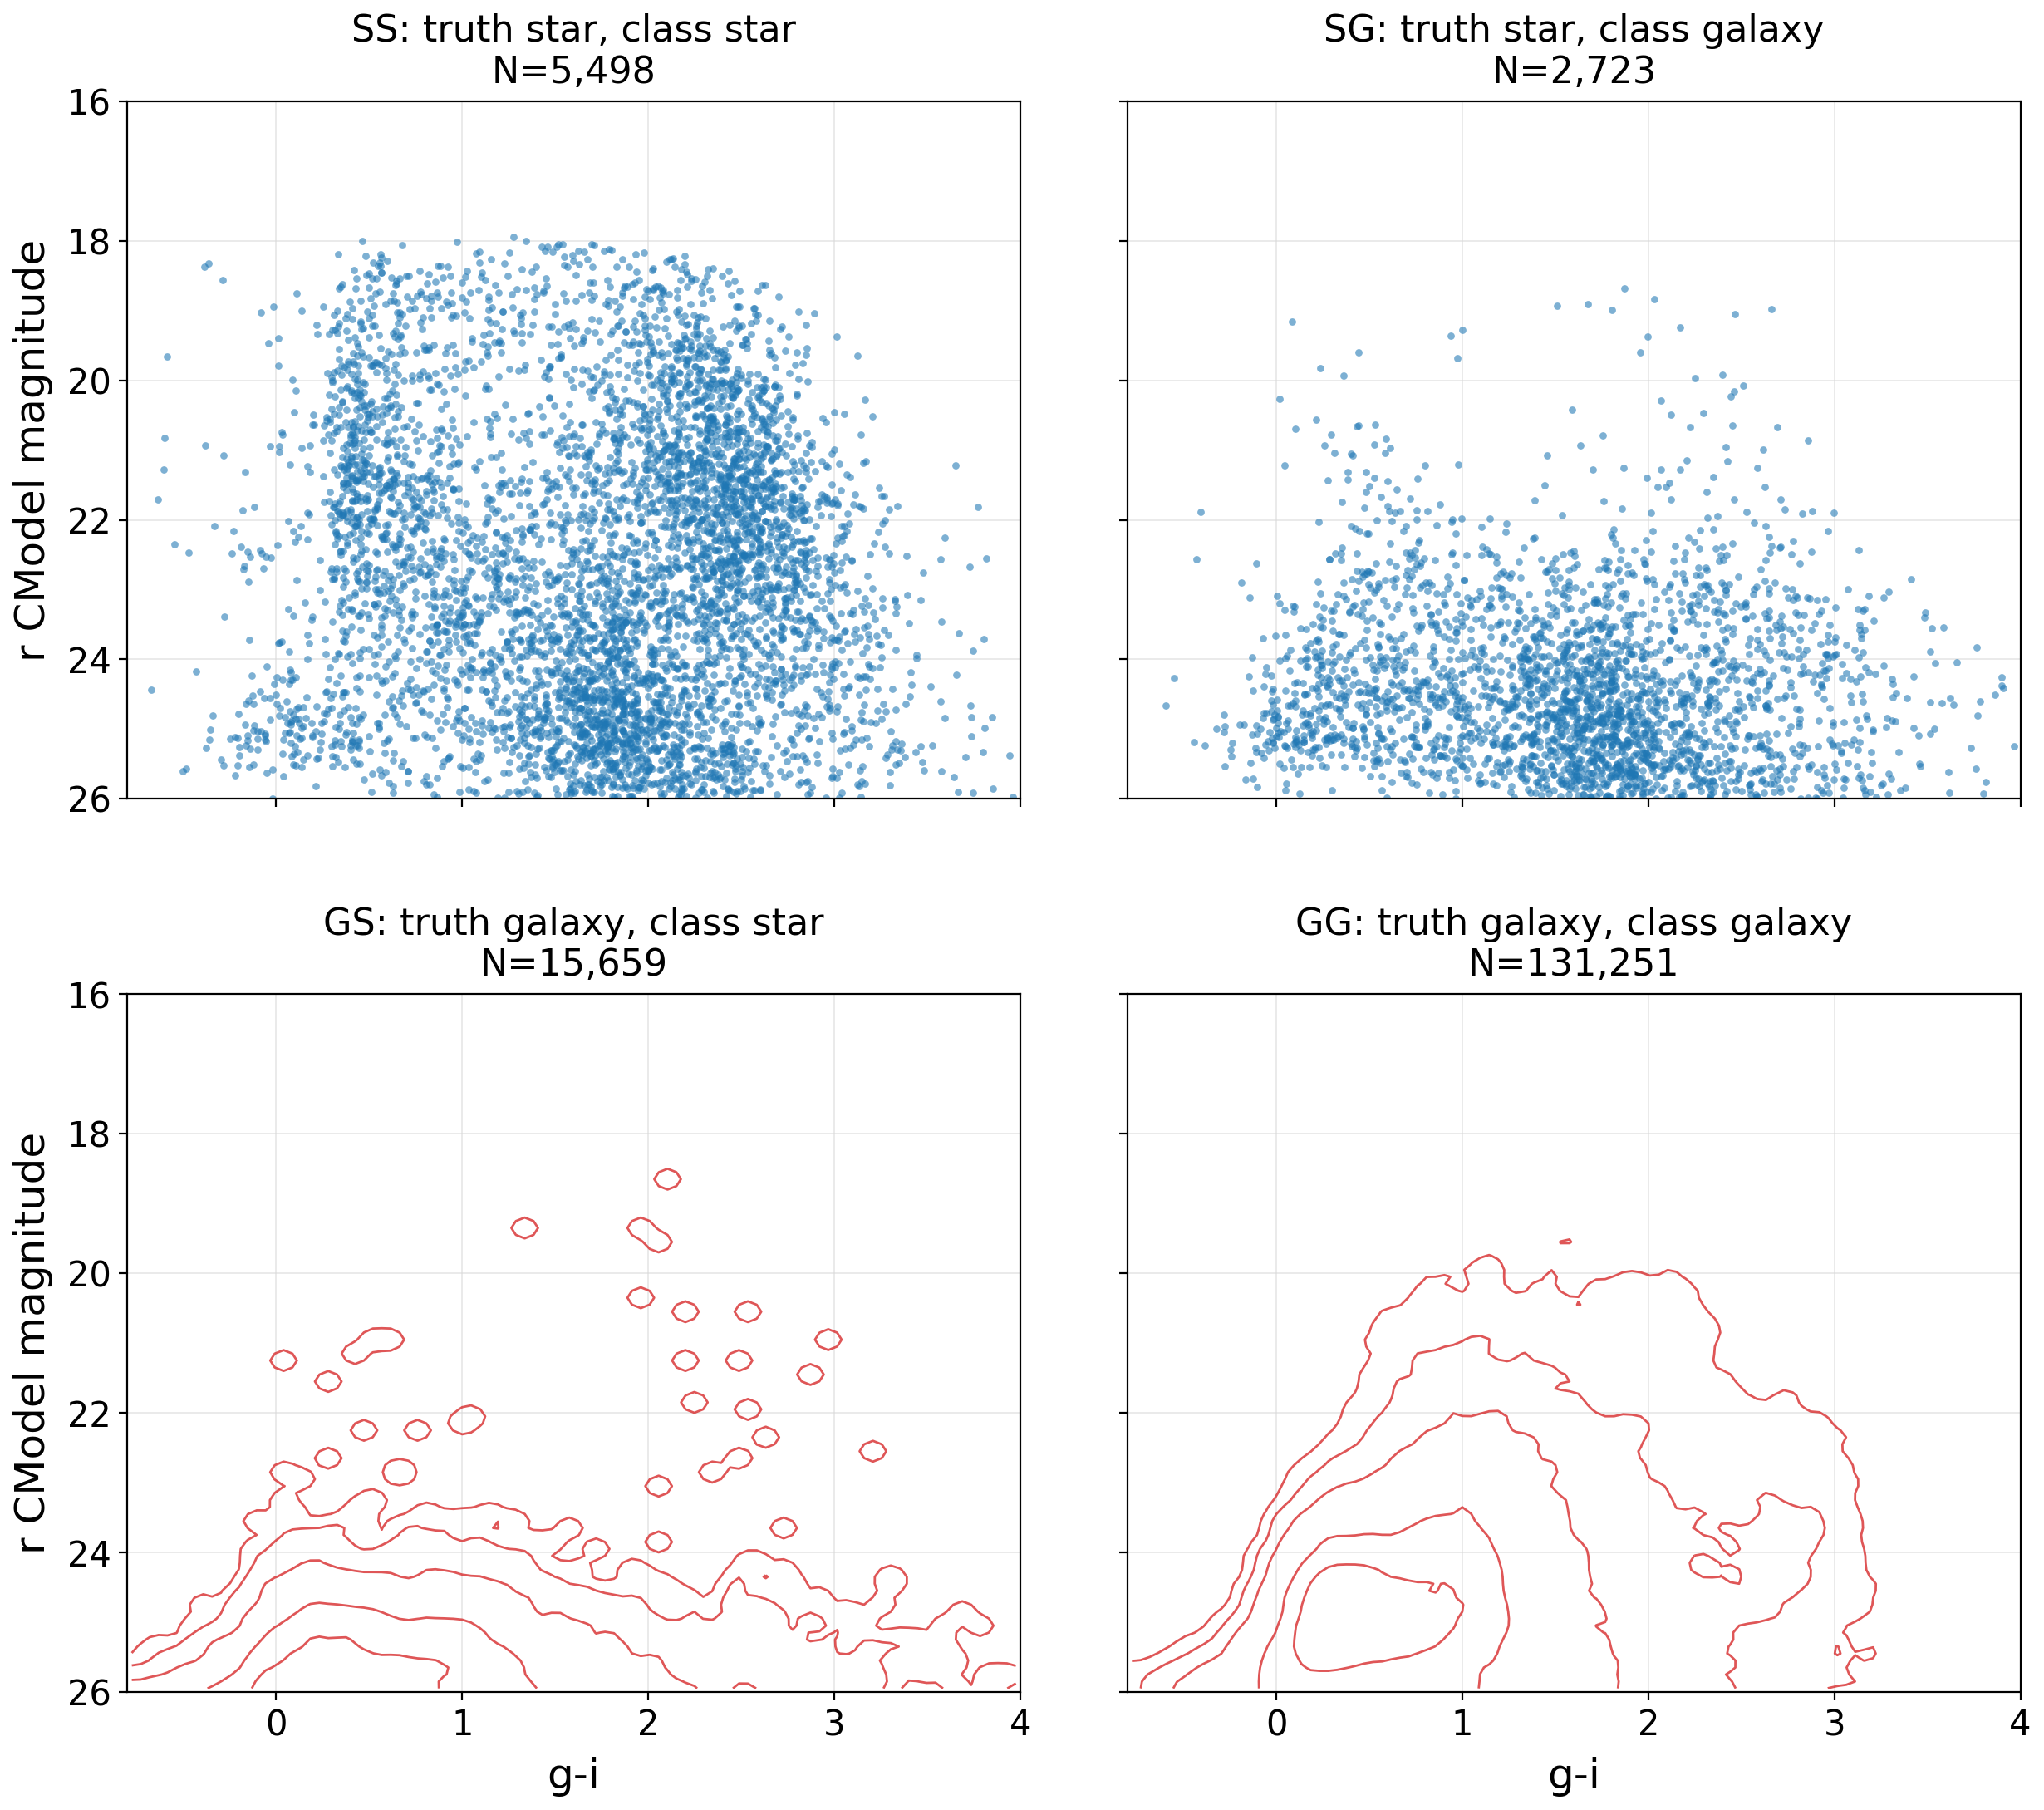
\includegraphics[width=\textwidth]{fig05_r_extendedness_confusion_cmd.png}
  \caption{Performance of Rubin's default \texttt{extendedness} parameter in the $r$ band
    relative to HST ground-truth labels. The top left and bottom right panels show
    correctly classified unresolved and resolved sources in the $r$ vs. $g-i$ color-magnitude
    diagram, with counts shown in the title above each panel. The bottom left and the top right panels
    show misclassified sources. Note that the stellar sample selected by \texttt{extendedness}=0
    is severely contaminated by galaxies for \(r_{\mathrm{CModel}} > 24\) (bottom left panel).}
  \label{fig:r_extendedness_confusion_cmd}
\end{figure*}



\subsection{Suspect HST Classification Labels} 
\label{sec:suspectHST}


There is a subset of objects classified as ``stars'' (unresolved) by HST which appear clearly
resolved when using Rubin's default \texttt{extendedness} parameter. Figure~\ref{fig:suspectHSTccd}
shows their distribution in color-color diagrams, with symbols color-coded by \(\Delta m \) in the
$r$ band. As evident, their color-color distribution is inconsistent with main stellar locus and similar
to that expected for barely resolved or unresolved binary stars (see Figures 2 and 4 in \citealt{2004ApJ...615L.141S}.)
To test this hypothesis, we visually inspected several hundred images (443 objects with HST label
``star'', $r<23$ and $\Delta m > 0.05$ mag; see Figure~\ref{fig:suspectHSTimages} for an example). 
Only 1.4\% of selected objects are detected as ``isolated'' (computed using processing flag
``detect\_isIsolated'') and about half seem to have a nearby stellar-like companion. In some cases a
bright source or an extended galaxy is nearby, and about one tenth or fewer appear bluish and
consistent with quasars. Detailed examination of such cases is beyond the scope of this work. 

Because we aim to test statistical performance of our star-galaxy separation method on unambiguous
objects, we exclude objects with HST ``star'' label that both appear resolved in Rubin data and also
have Rubin colors inconsistent with the main stellar locus. 

{\bf DANIEL:} can you please add a paragraph here about how you rejected some HST stars by colors
and what were the numbers (fractions) of rejected objects (and how you handled variation with
magnitude)?  


\begin{figure*}
  \centering
  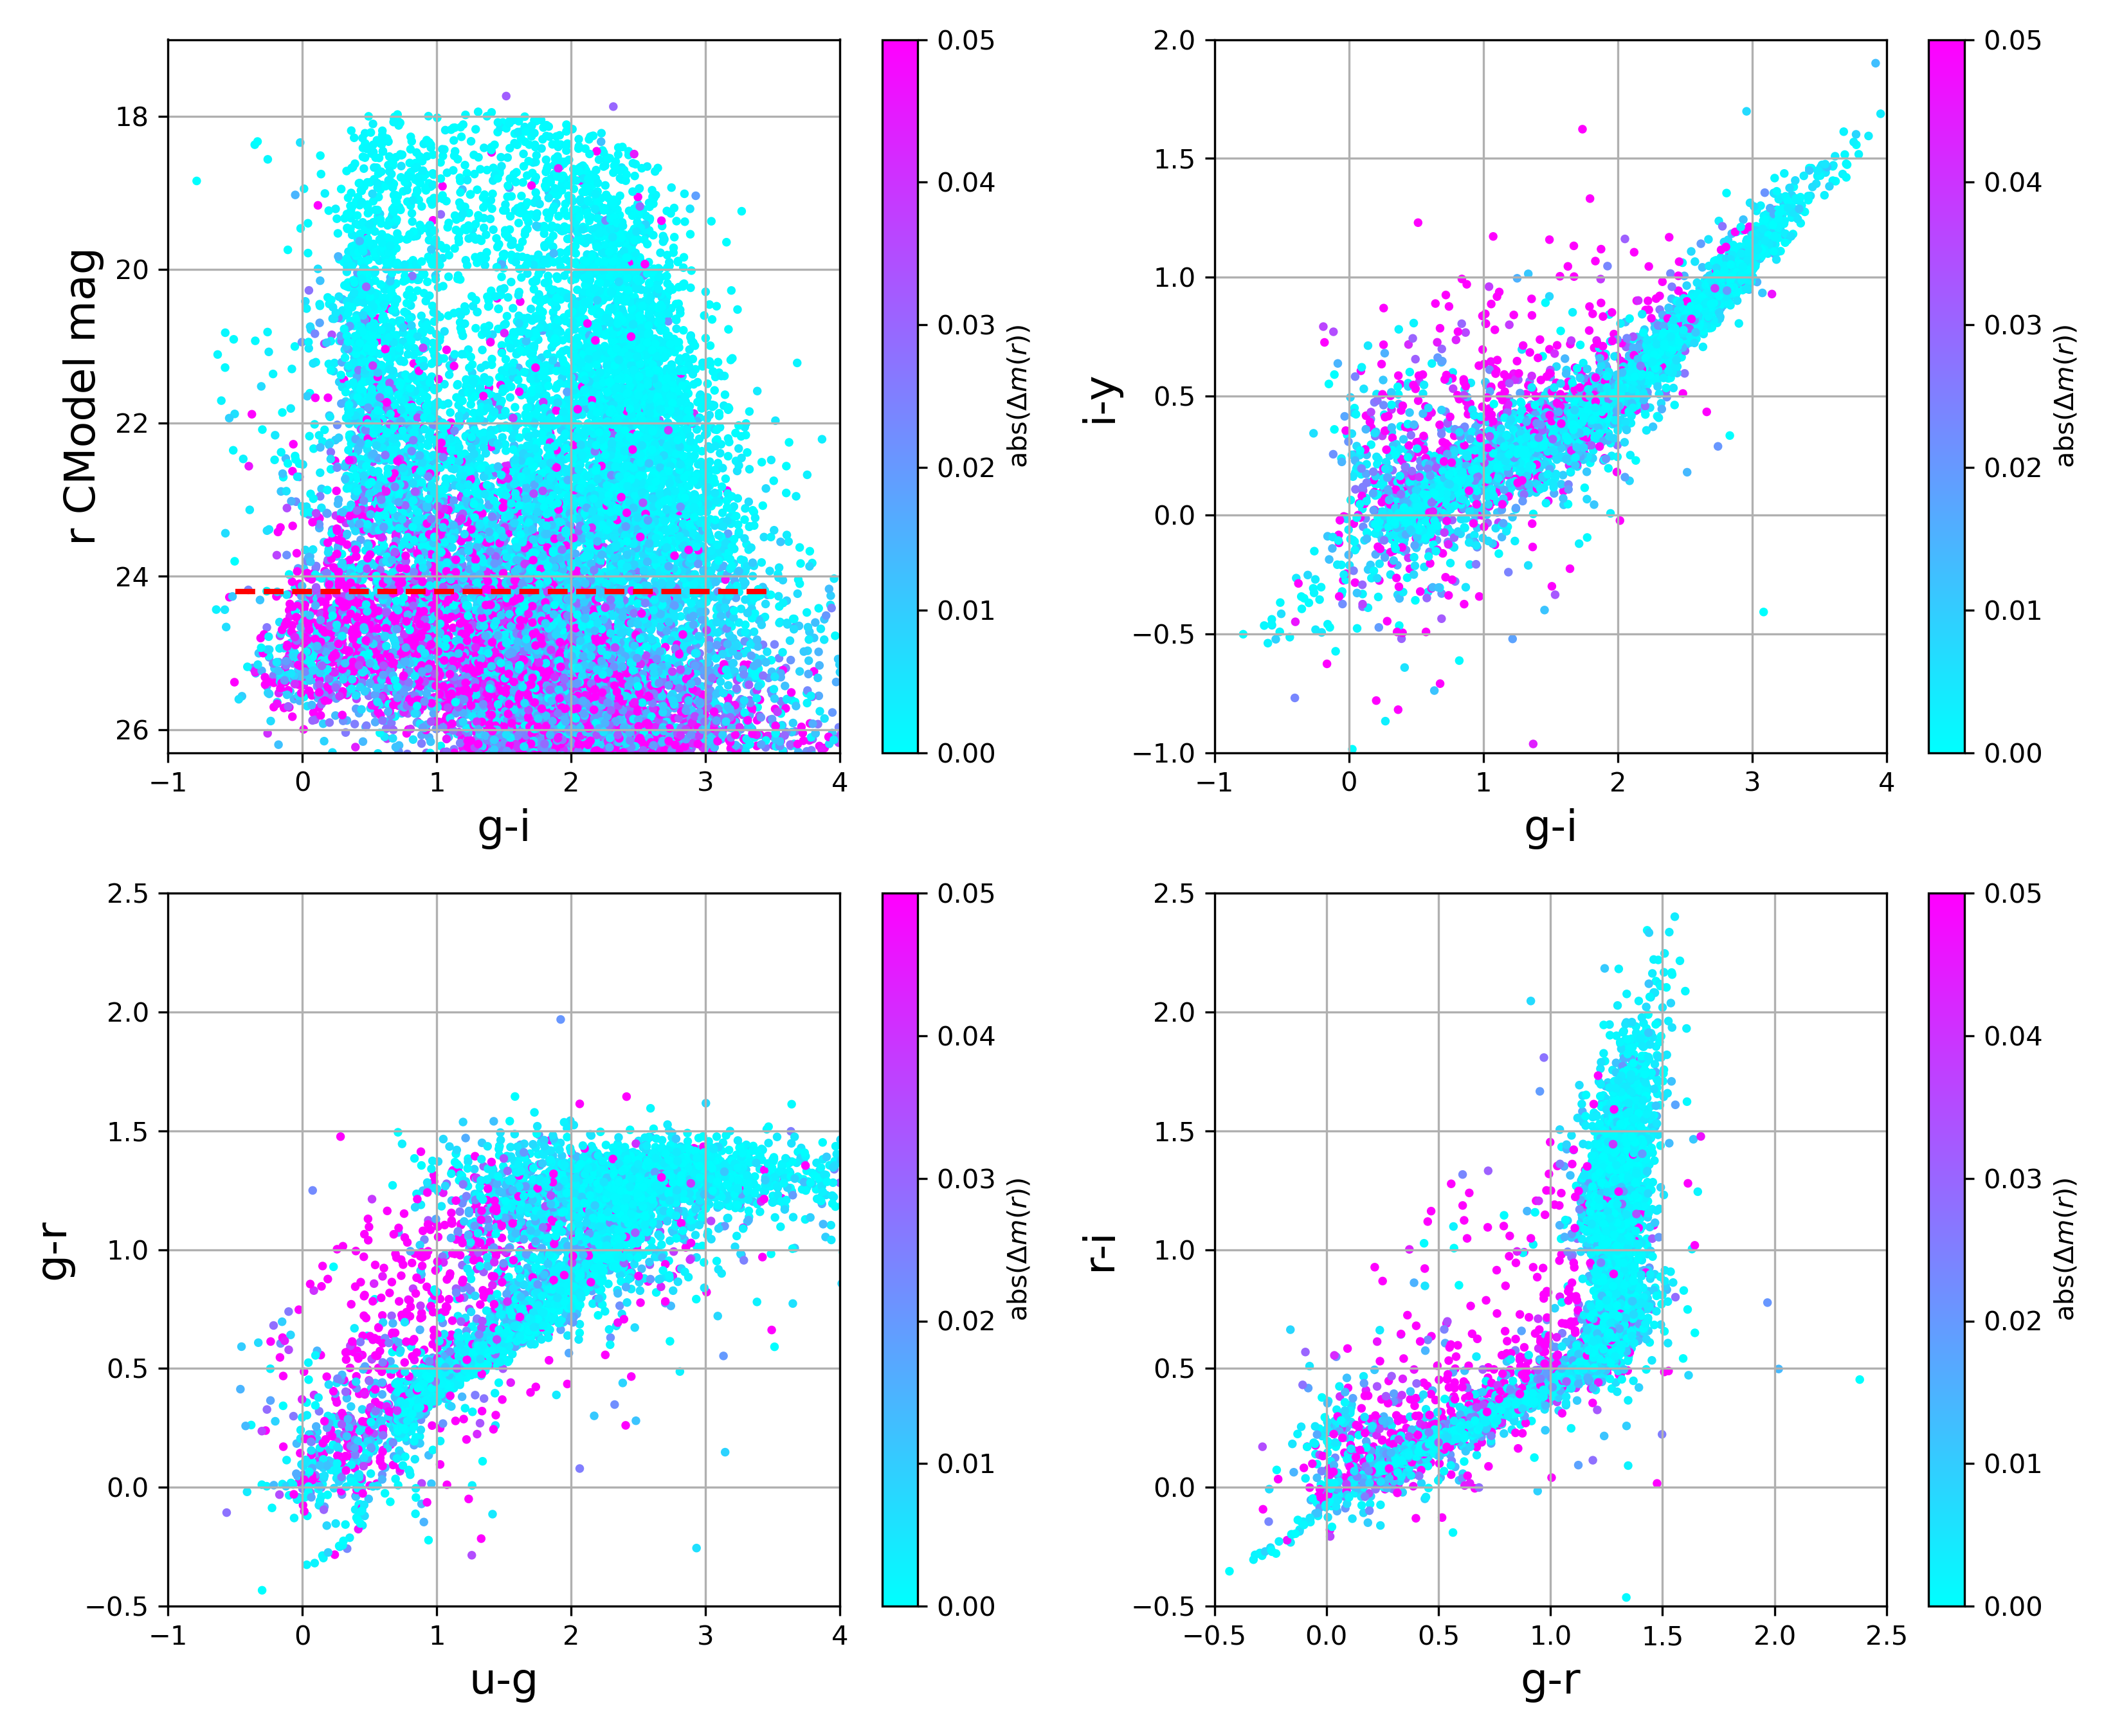
\includegraphics[width=0.9\textwidth]{COSMOSdm_HSTstarColored.png}
  \caption{The distribution of objects classified as ``stars'' by HST, but which appear clearly
    resolved when using Rubin's default \texttt{extendedness} parameter, in color-magnitude
    (top left) and informative color-color diagrams. Only objects with $r < 24.2$ are shown
    in the three color-color diagrams. Symbols are color-coded by the absolute value of
    Rubin's \(\Delta m \) in the $r$ band.  The color-color distribution of objects with
    $|\Delta m| > 0.05$ mag (about 3\% of all objects classified by HST as ``stars'' and brighter
    than $r=23$) is inconsistent with main stellar locus and similar to that expected for barely
    resolved or unresolved binary stars. 
}
  \label{fig:suspectHSTccd}
\end{figure*}



\begin{figure*}
  \centering
  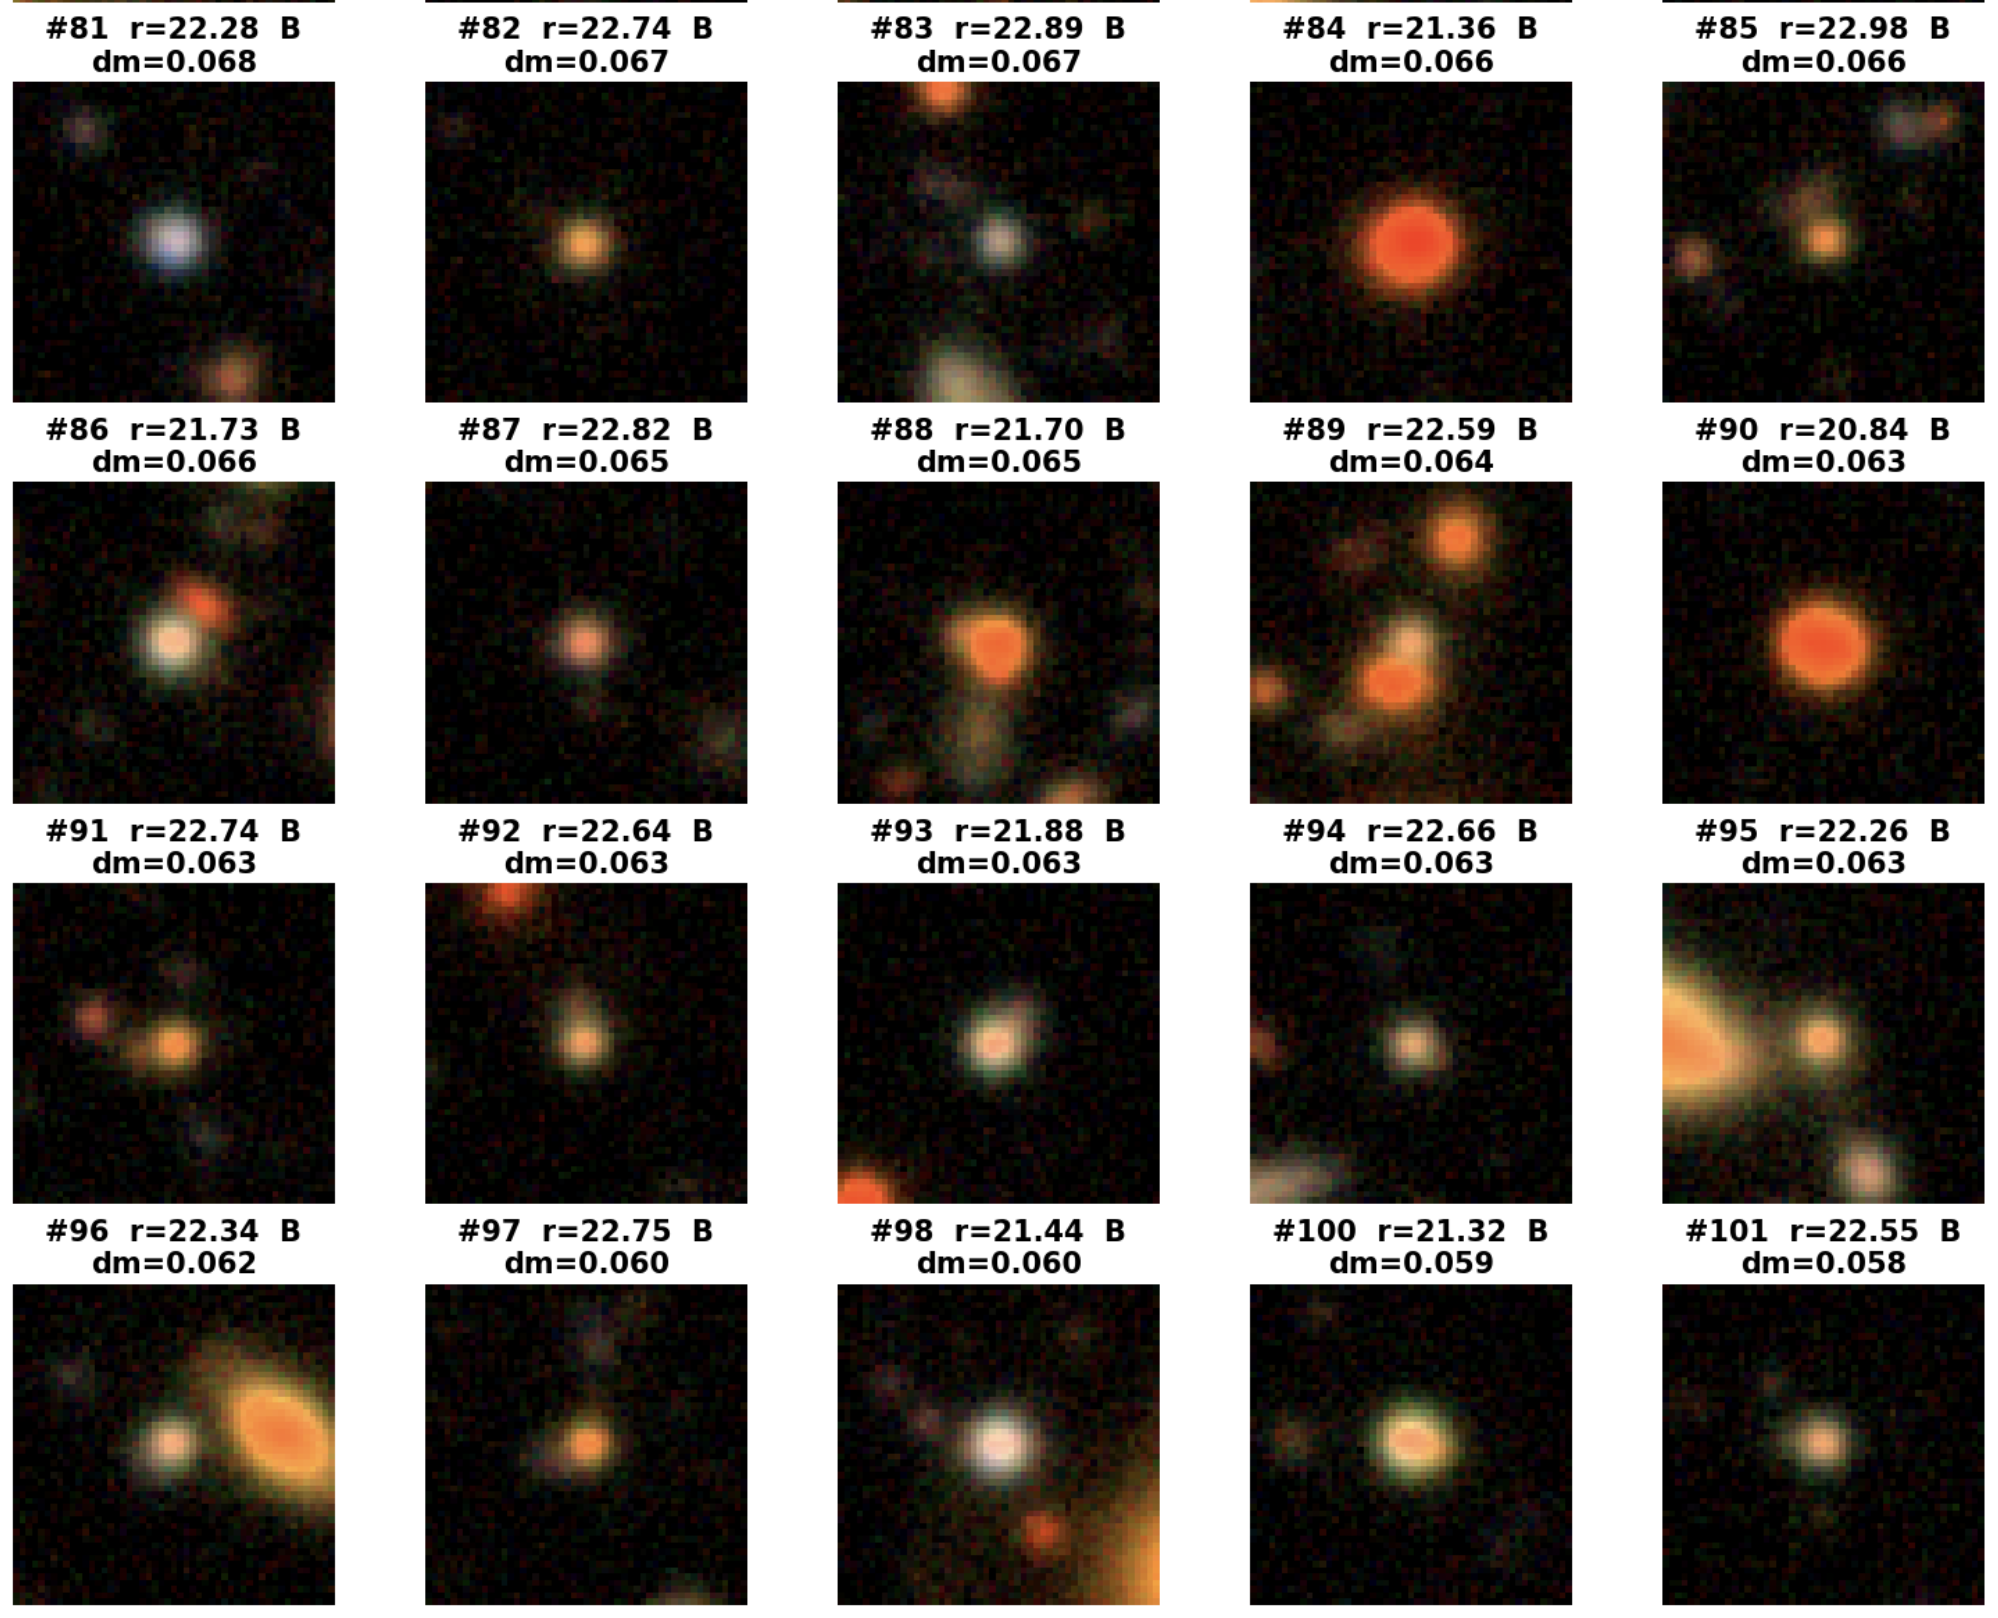
\includegraphics[width=\textwidth]{suspectHSTimages.png}
  \caption{The Rubin $gri$ color composite images extracted from ``deep\_coadd'', 10 arcsec by
    10 arcsec (50x50 pixels), for a random subsample of 443 objects selected as ``stars'' in HST and
    resolved in Rubin, and brighter than $r=23$. About 98.6\% are detected as blended objects.} 
  \label{fig:suspectHSTimages}
\end{figure*}
 

\appendix{A toy model for $D$ distributions}

Here we describe toy model... Figures ~\ref{fig:toymodel1} and ~\ref{fig:toymodel2}


\begin{figure*}
  \centering
  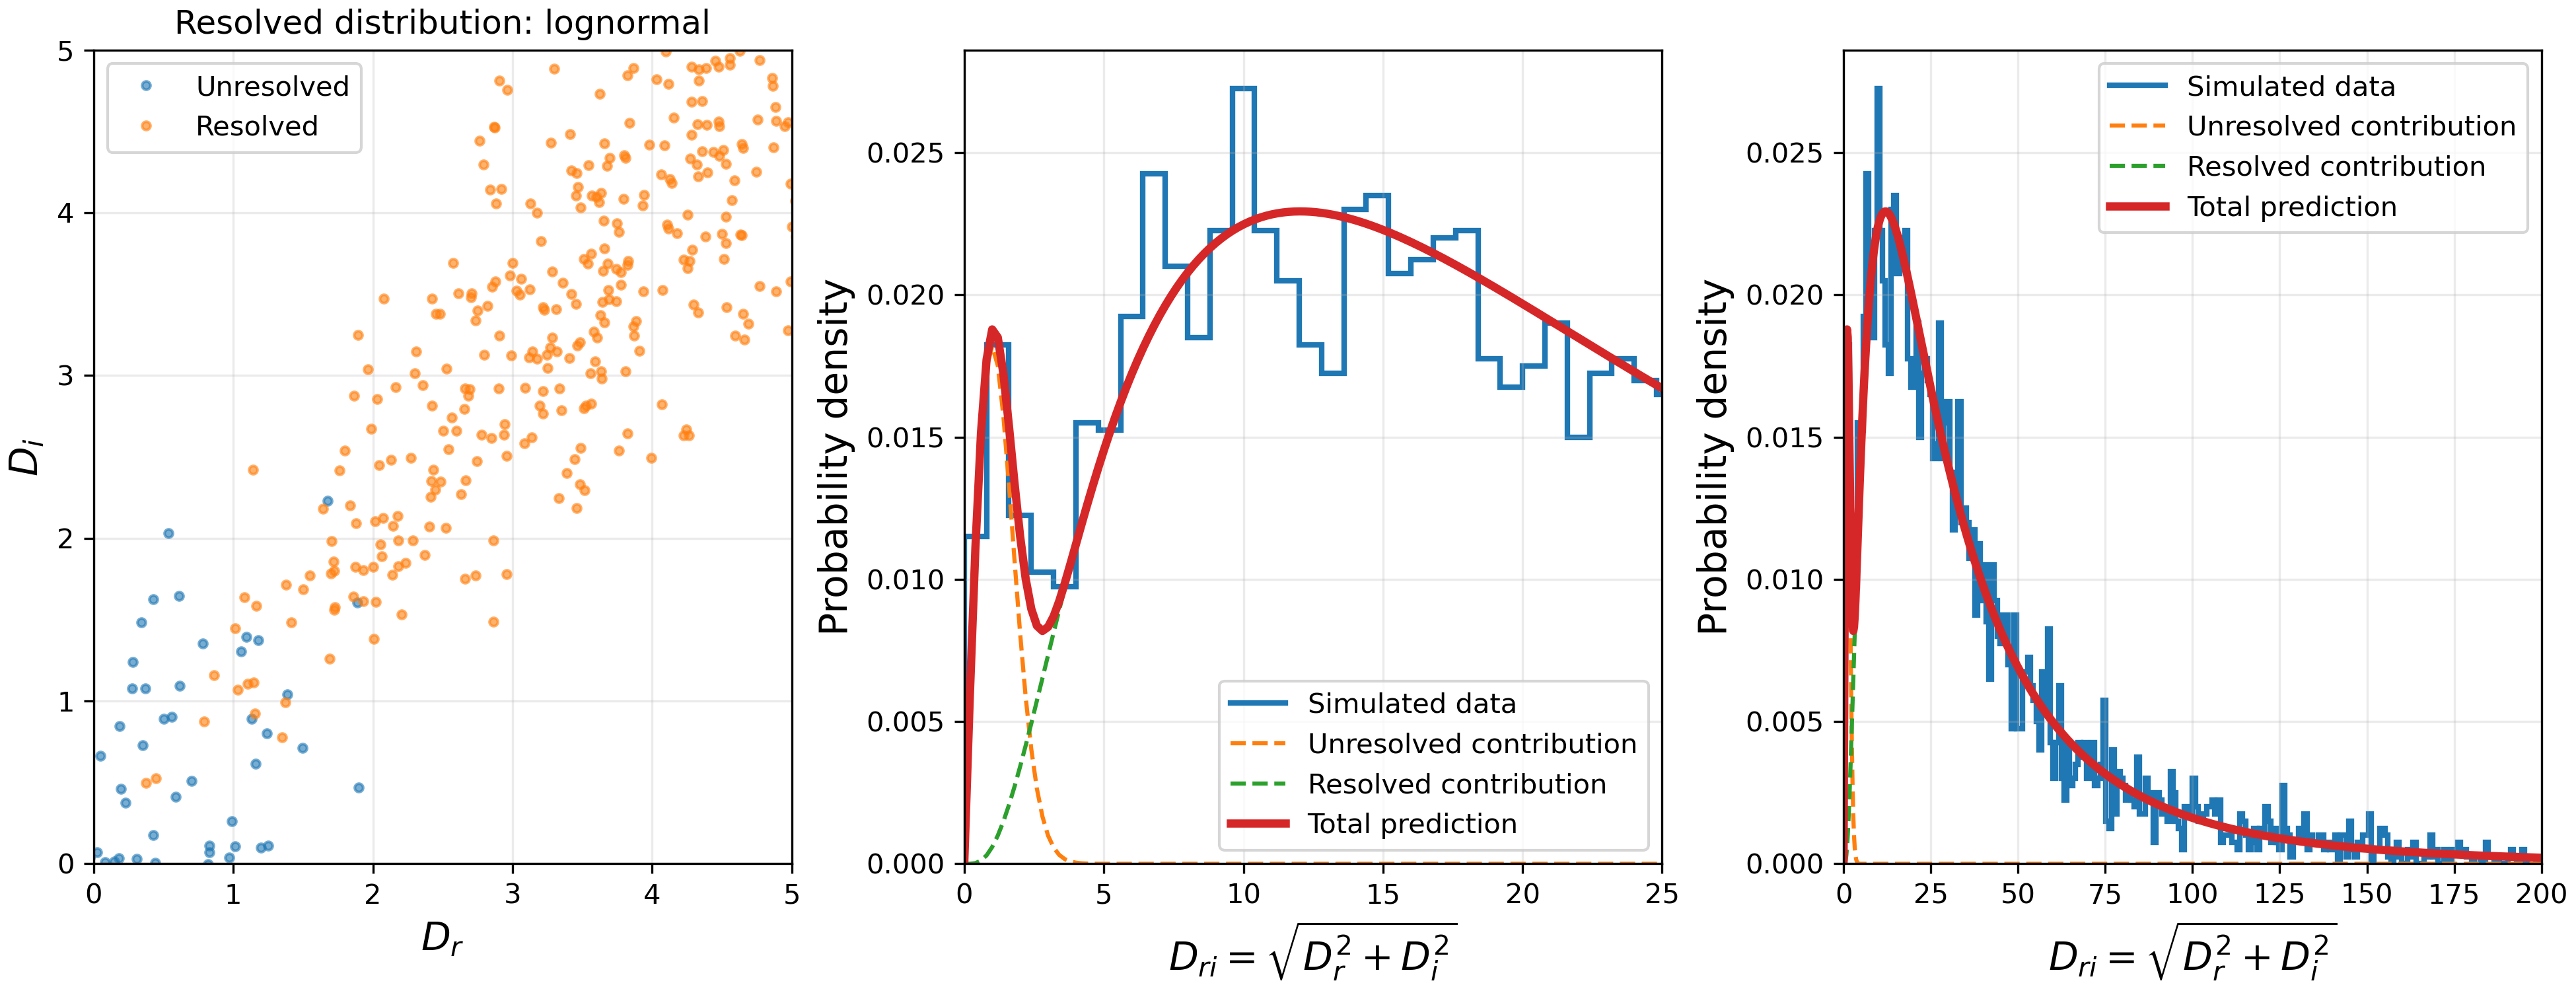
\includegraphics[width=\textwidth]{simulate_and_plot.png}
  \caption{First figure...}
  \label{fig:toymodel1}
\end{figure*}


\begin{figure*}
  \centering
  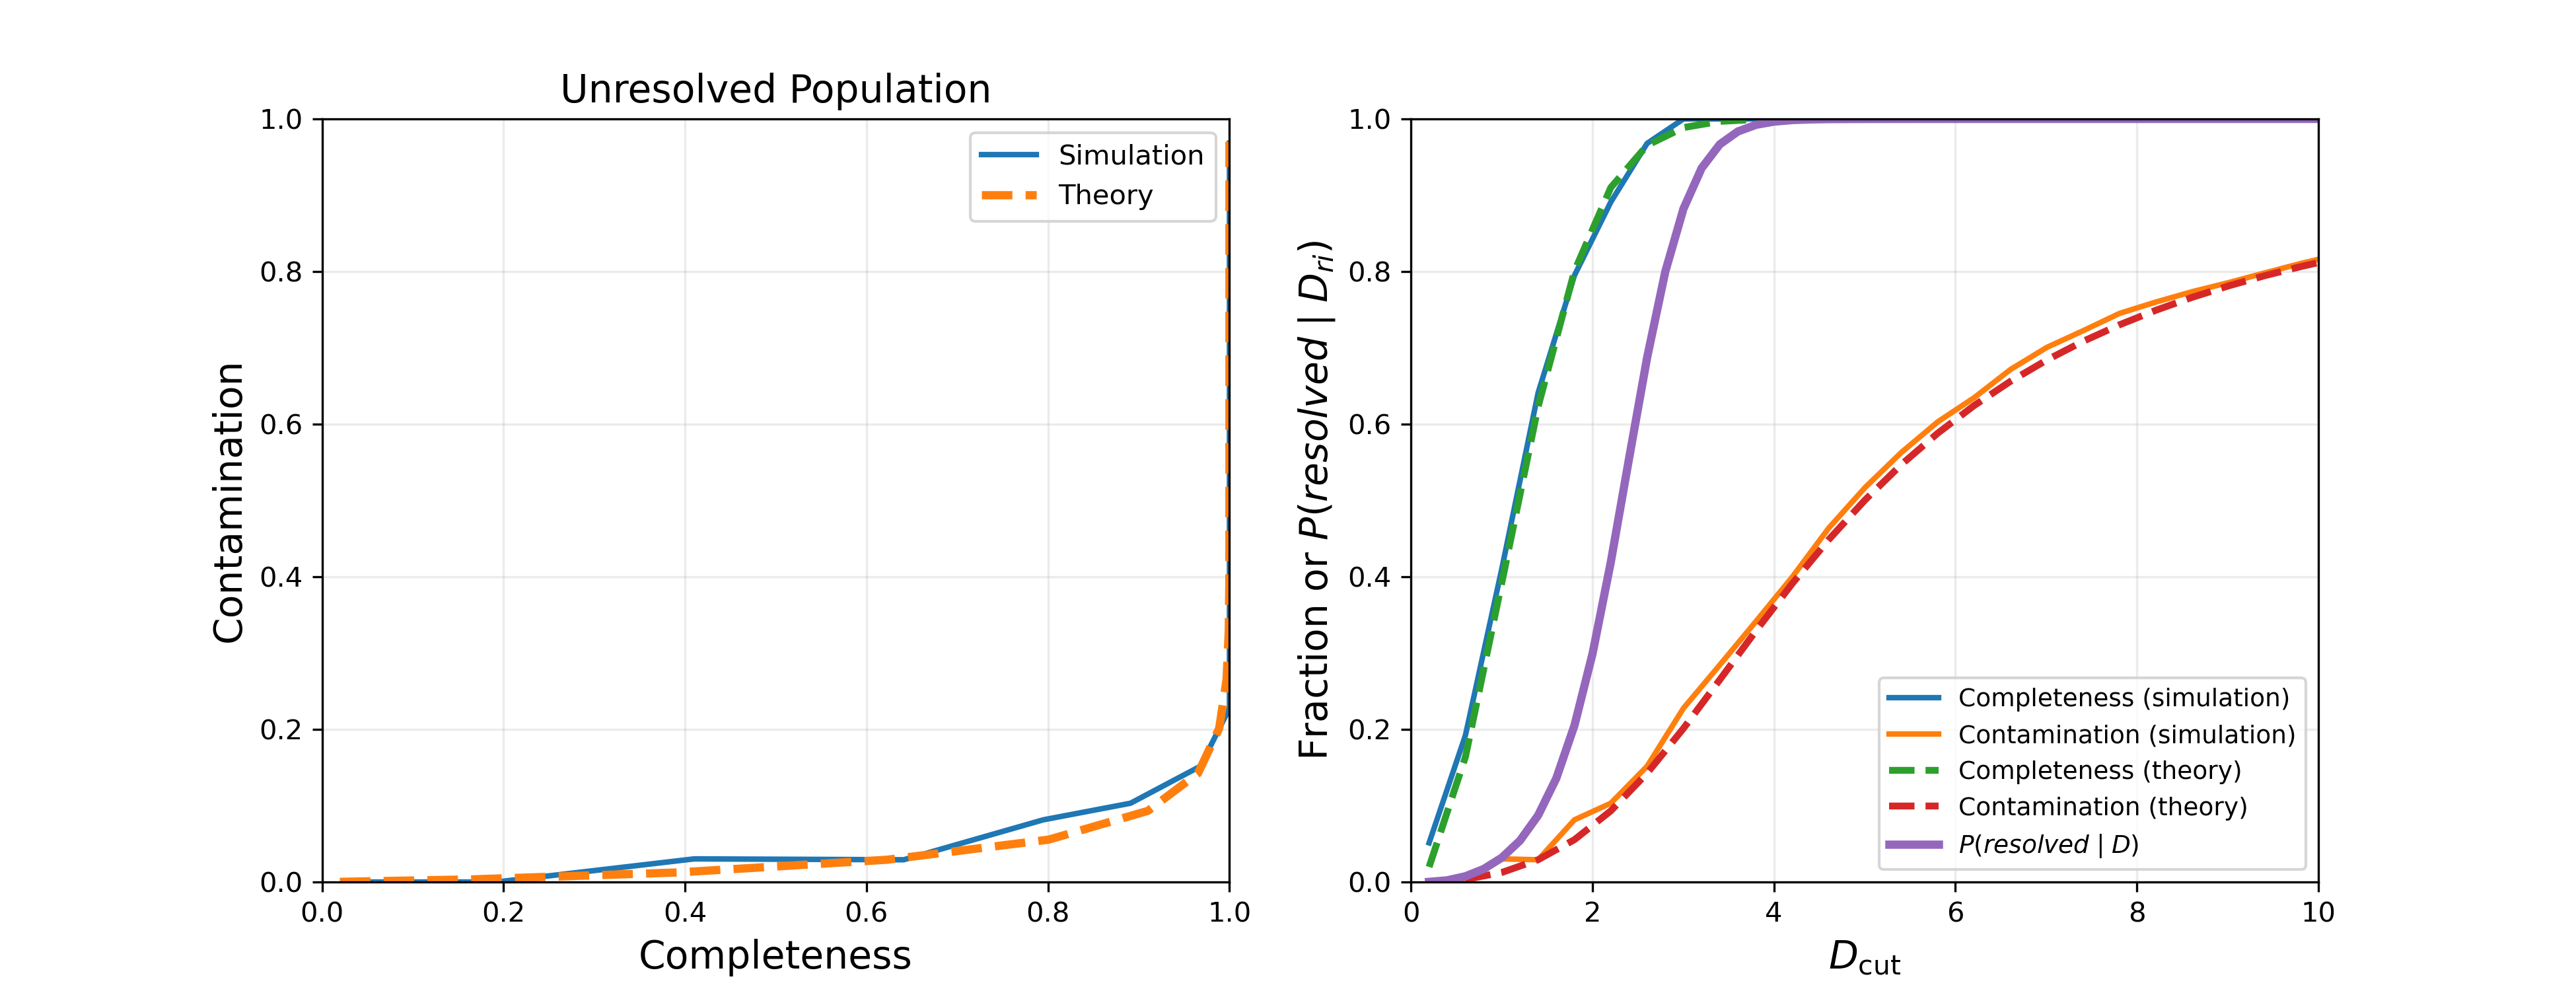
\includegraphics[width=\textwidth]{simulation_vs_theory.png}
  \caption{Second figure...}
  \label{fig:toymodel2}
\end{figure*}


 


% 
\section{Star-galaxy Separation Methodology}

We first briefly review the Bayesian star-galaxy separation method proposed in SIL2020 and then
apply it to single-band Rubin data, followed by its extension to multi-band case. Our principal
measured object property is the difference between PSF, \(m_{\mathrm{PSF}}\), and CModel, \(m_{\mathrm{CModel}}\),
magnitudes, \(\Delta m = m_{\mathrm{PSF}} - m_{\mathrm{CModel}}\). For unresolved sources, this \(\Delta m \)
is vanishing within noise, while for resolved objects \(\Delta m > 0\) (see Figure~\ref{fig:truth_morphology_color}).
A comparison and statistical discussion of this quantity and several other quantities proposed for
star-galaxy separation in the literature is available in SIL2020. 



\subsection{Bayesian Star-Galaxy Separation Method from SIL2020}

We first focus on the single-band case and then will extend our discussion to then multi-band case.
SIL2020 showed using realistic simulations that adopting a fixed pre-defined threshold for $\Delta
m$ in order to select resolved objects is not optimal. Not only that this threshold should depend
on magnitude due to variation of object populations, signal-to-noise ratio due to statistical noise,
and sky location due to varying count ratio of galaxies and stars, but for optimal combination of
information from different bands, or from other classification methods (e.g., based on colors),
observed $\Delta m$ distribution needs to be transformed into a proper probability density function. 

The subsample of objects with HST labels can be used to quantify $\Delta m$ distribution separately
for unresolved and resolved objects. However, such a ``training'' sample is currently available only
for a very small fraction of LSST footprint (less than 1\% of the area). Instead, we use the fact
that very large numbers of objects that remain even after binning in both sky location and magnitude
can robustly constrain two components of $\Delta m$ distribution even when such labels are not
available a priori. We only use the subsample of objects with HST labels to independently assess the
performance of our method. 


\subsection{Mixture Model for \(\Delta m\) vs. \(m_{\mathrm{CModel}}\) diagram \label{sec:mixmodel}} 

We assume that a sample is selected from a judiciously chosen sky region over which the variation
of stellar and galaxy population can be assumed statistically uniform. Over angular scales of
several degrees, stellar counts vary much more rapidly than galaxy counts (large galaxy clusters are
an exception but not important for subsequent discussion). Based on the analysis of state-of-the-art
Milky Way stellar population models by \cite{2025AJ....169..119P}, a sky region of several square
degrees, corresponding to Rubin tracts\footnote{In the Rubin Science Pipelines, tracts and patches
are the two levels of spatial subdivision used for coadded images and object catalogs. They are
designed to make processing and storage scalable while preserving continuity across the sky.
A tract is a relatively large region of the sky, approximately 1.75$^\circ$ x 1.75$^\circ$ (the exact
size depends on the sky map projection). that is processed as a unit. Tracts overlap slightly with
neighboring tracts to avoid edge effects. Each tract is subdivided into a regular grid of patches,
with each tract in DP2 containing 81 patches. The patch size is about 12 arcmin by 12 arcmin
(approximately, one CCD).}  is sufficiently small for this purpose (and consistent with our choice of
the COSMOS field for quantitative analysis). 
 
Given a ``tract'' catalog, and at a fixed CModel magnitude (see below for binning details), the
distribution of \(\Delta m\) in a given band (not explicitly marked for notational simplicity) is
modeled as a mixture of an unresolved (star) component and a resolved (galaxy) component, 
\begin{equation}
                                p(\dm \,|\, m) = w_U \, \funr (\dm) +  w_R \, \fres (\dm),
  \label{eq:mixpdf1}
\end{equation}
where $w_U + w_R = 1$, and $\funr$  and $\fres$  are properly normalized probability density
functions. With this decomposition, the probability that an object is unresolved is given by
Bayes' theorem as
\begin{equation}
        p_S(\dm) =p({\rm unr}\mid\dm)= \frac{w_U \funr(\dm)}  {w_U \funr (\dm) + w_R \fres (\dm)}.
  \label{eq:pSdm} 
\end{equation}
and the probability that it is resolved is $p_G = 1 - p_S$ (note that we use indices $S$ and
$unr$, or $G$ and $res$ interchangeably). 

The same model predicts the performance, the completeness and contamination for each class,
as function of a hard $\dm$ threshold. If $\dm<\dm_{\rm cut}$ is classified as unresolved,
\begin{equation}
                           {\rm Completeness}_S= \int_{-\infty}^{\dm_{\rm cut}}\funr (\dm) d\dm,
\end{equation}
and
\begin{equation}
                          {\rm Contamination}_S = \frac{w_U  \int_{-\infty}^{\dm_{\rm cut}}\funr (\dm) d\dm}
     {w_U \int_{-\infty}^{\dm_{\rm cut}}\funr (\dm) d\dm  + w_R \int_{-\infty}^{\dm_{\rm cut}}\fres (\dm) d\dm}.
\end{equation}
We test these predictions below using HST-based labels.
% However, one needs to be careful because HST labels are not perfect.
% There are HST stars that appear resolved in Rubin and have non-stellar colors (quasars, close
%  binary stars) and some HST galaxies are cannot be resolved using Rubin images obtained with
%  ground-based seeing.

Therefore, a good model for $p(\dm \,|\, m)$ (eq.~\ref{eq:mixpdf1}) is crucial. Informed by observed
$\dm$ distributions, we model the unresolved component, $\funr$ as a single Gaussian with mean
\(\mu_U\), width \(\sigma_U\) (and weight \(w_U\)).  The resolved component is modeled as a sum
of \(K\) log-normal distributions with weight \(w_{R,k}\), location
\(\mu_{R,k}\), scale \(\sigma_{R,k}\), and shape parameter \(\alpha_{R,k}\). The full
mixture probability density function is
\begin{equation}
  p(\Delta m \,|\, m) = w_U \, \mathcal{N}(\Delta m | \, \mu_U,\, \sigma_U)
    + \sum_{k=1}^{K} w_{R,k} \, \mathcal{LN}(\Delta m | \, \mu_{R,k},\, \sigma_{R,k},\, \alpha_{R,k}),
  \label{eq:mixture_pdf}
\end{equation}
where \(\mathcal{N}\) denotes the Gaussian and \(\mathcal{LN}\) the log-normal distribution,
and the weights are constrained to sum to unity: \(w_U = 1 - \sum_k w_{R,k}\) (functions
\(\mathcal{N}\) and \(\mathcal{LN}\) are properly normalized probability density functions).
The galaxy-to-star count ratio, which serves as Bayesian prior, is equal to
\begin{equation}
                   N_{GS} \equiv   {N_G \over N_S}  = {\sum_{k=1}^{K} w_{R,k}  \over  w_U}. 
\end{equation}
The expression given by eq.~\ref{eq:pSdm} can be recast as
\begin{equation}
              p_S(\dm) =   \frac{1}  {1 +  N_{GS}  \, BF},
  \label{eq:pSbf} 
\end{equation}
where Bayes factor is equal to
\begin{equation}
              BF = \frac{\fres} {\funr}. 
  \label{eq:bfdef} 
\end{equation}
With $N_{GS} \sim 30$ (see Figure~\ref{fig:star_galaxy_ratio_v8v9}), it is sufficient to have $BF \sim 0.033$
for $p_S$ to drop below 0.5 (because the sample is highly imbalanced).  This decomposition in terms of prior
and Bayes factor will be important later when combining multiple sources of classification information.  


\subsubsection{Fitting Details}

The fitting is performed independently in bins of CModel magnitude. At bright magnitudes
(\(m_{\mathrm{CModel}} < 22\)), where the resolved population is relatively simple, we use
\(K = 2\) resolved components in bins of width 1--3~mag spanning
\(15 < m_{\mathrm{CModel}} < 22\). At faint magnitudes (\(m_{\mathrm{CModel}} \geq 22\)),
where the galaxy morphology distribution is more complex, we use \(K = 3\) resolved components
in finer bins of width 0.5--1~mag spanning \(22 \leq m_{\mathrm{CModel}} < 27\). Within each
magnitude bin, \(\Delta m\) values in the range \((-0.5, 1.5)\) are binned into 300 bins
and normalized to unity. The mixture model is fit to these histograms using
bounded least-squares optimization with Poisson-like uncertainties
\(\sigma_i = \sqrt{N_i + 1} \,/\, (N \, \delta)\), where \(N_i\) is the count in bin \(i\),
\(N\) is the total number of sources in the magnitude slice, and \(\delta\) is the histogram
bin width.

This fitting procedure is carried out in three steps. In the first step, all mixture parameters
are fit independently in each magnitude bin. This free fit works well at bright magnitudes,
where unresolved and resolved sources are clearly separated in \(\Delta m\). However, at faint
magnitudes (\(m_{\mathrm{CModel}} \gtrsim 24\)), photometric noise broadens the unresolved
Gaussian until it becomes degenerate with the resolved components. The fitter can no longer
reliably distinguish the two populations, causing the unresolved Gaussian to absorb flux from
the galaxy distribution. This inflates the inferred star fraction at faint magnitudes.

To prevent this degeneracy, we impose smooth constraints on the unresolved component.
In the second step, the per-bin star parameters from step~1 are replaced with smooth
functions of magnitude: \(\mu_U\) is fixed to a single value (the median across all bins,
typically \(\approx 0\) in each band); \(\sigma_U(m)\) is fit with the photometric error model
from \citet{2007AJ....134.2236S} (their eq.~5),
\begin{equation}
  \sigma_U(m) = \sqrt{\sigma_0^2 + a^2 \cdot 10^{\,b\,(m - 25)}},
  \label{eq:sesar_sigma}
\end{equation}
where \(\sigma_0\), \(a\), and \(b\) are free parameters; and \(w_U(m)\) is modeled as a linear
fit to \(\log_{10}(w_U)\) versus magnitude, using only bins brighter than
\(m_{\mathrm{CModel}} = 24\) where the free fit is reliable. This smooth model is then
extrapolated to fainter magnitude bins. In the third step, with the unresolved component
(\(\mu_U\), \(\sigma_U\), \(w_U\)) fixed to the smooth curves from step~2, only the resolved
log-normal parameters are re-fit in each magnitude bin. The resolved weights are rescaled to
sum to \((1 - w_U)\) so that the total mixture remains a proper probability density.
The effectiveness of this constrained fitting procedure is demonstrated in
Figure~\ref{fig:star_galaxy_ratio_v8v9}, which compares the galaxy-to-star count ratio
\(\log_{10}(N_{\mathrm{gal}}/N_{\mathrm{star}})\) as a function of magnitude for models
with and without the smooth constraints. The unconstrained model exhibits a spurious turnover
at faint magnitudes, while the constrained model recovers the expected monotonically increasing
ratio in agreement with the COSMOS2020 external truth labels (note that in this sample at the faint
end galaxies outnumber stars by more than a factor of 30). 

\begin{figure*} 
  \centering
  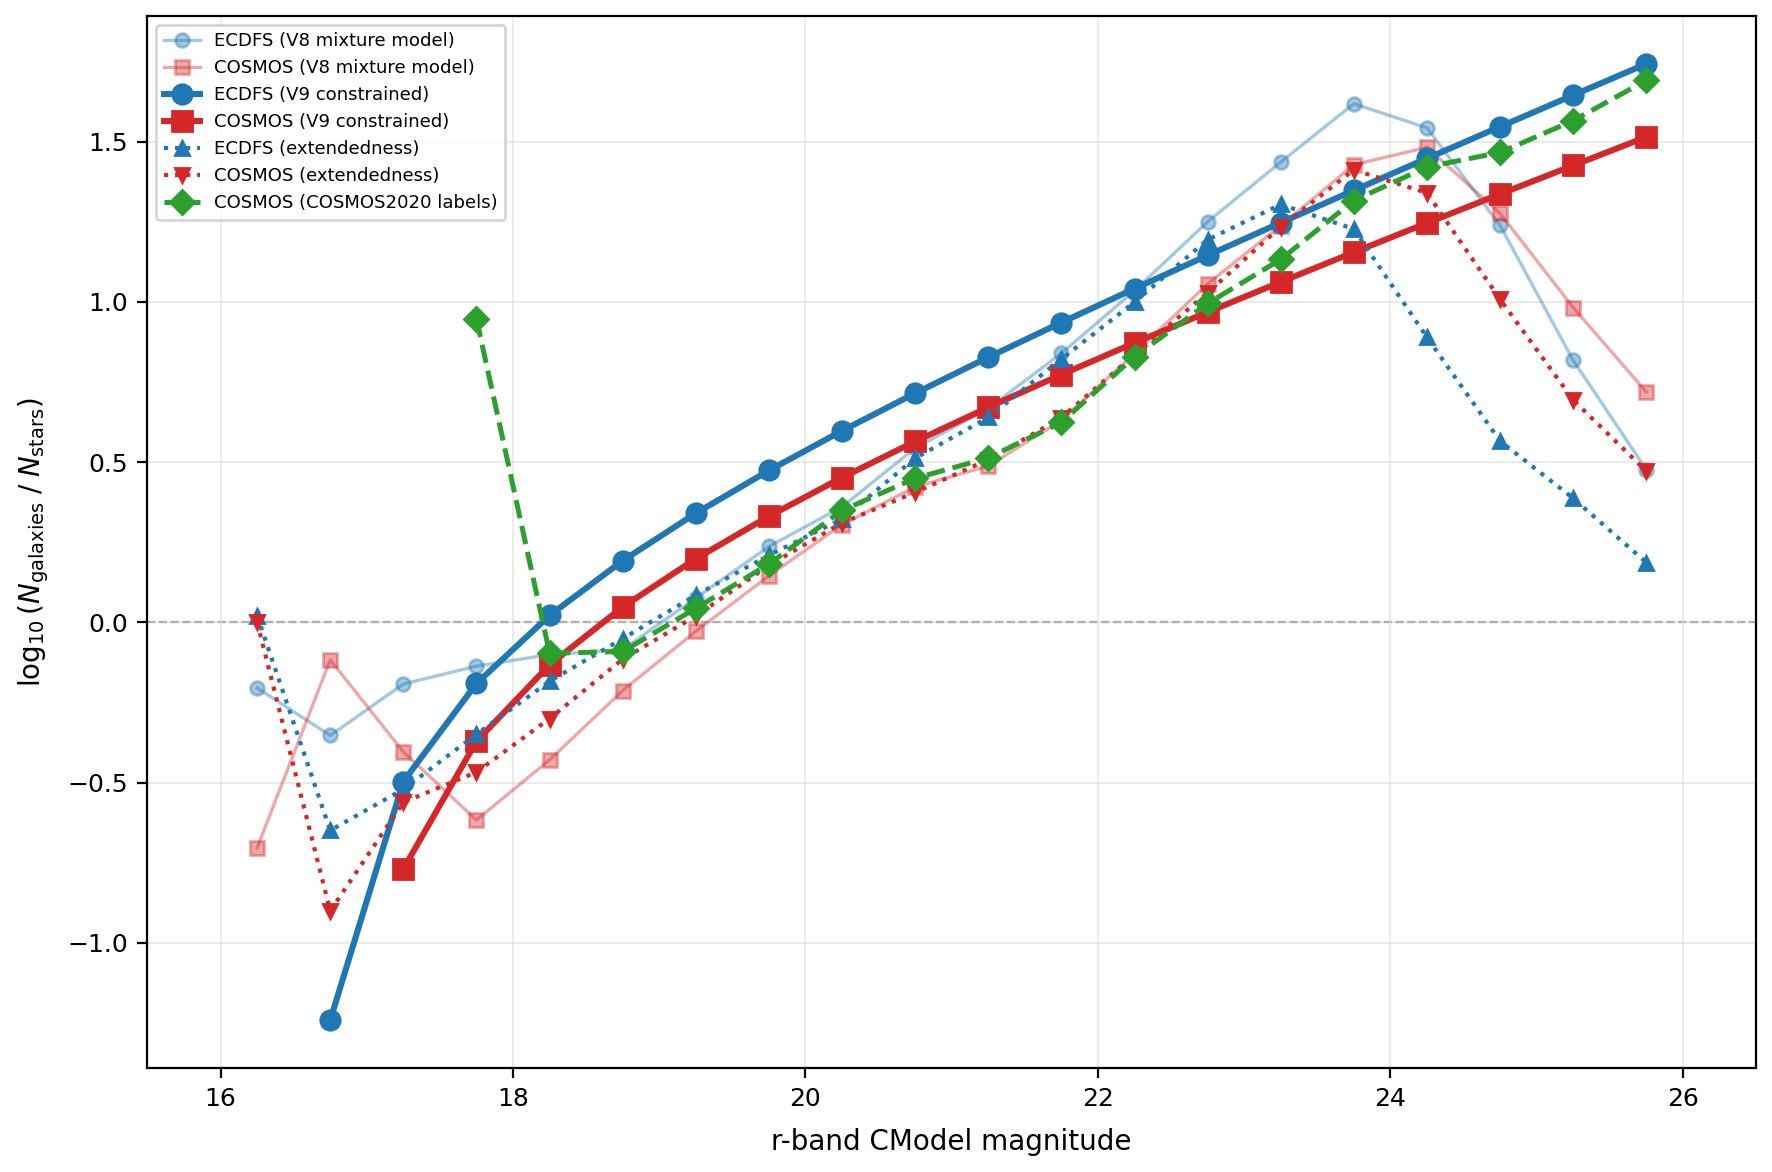
\includegraphics[width=\textwidth,height=0.62\textheight,keepaspectratio]{fig06_star_galaxy_ratio_vs_rmag_v8v9.png}
   \caption{Galaxy-to-star count ratio \(\log_{10}(N_{\mathrm{gal}}/N_{\mathrm{star}})\) vs.\
    r-band CModel magnitude. The unconstrained mixture model (marked V8, faded curves) exhibits a
    spurious turnover at \(m \gtrsim 24\) due to the unresolved Gaussian absorbing galaxy flux.
    The constrained model (marked V9, bold curves) recovers the expected monotonically increasing
    ratio, in good agreement with the COSMOS2020 truth labels (green dashed). Dotted lines show
    the Rubin \texttt{extendedness}-based classification for comparison (which also shows spurious
    turnover at the faint end.}
  \label{fig:star_galaxy_ratio_v8v9}
\end{figure*}

The model parameters are looked up by the CModel magnitude bin in which each source falls.
The quality of the fits is illustrated in Figure~\ref{fig:slice_fits}, which shows the
mixture model overlaid on the observed \(\Delta m\) histograms in each magnitude bin, and in
Figure~\ref{fig:model2d_residuals}, which shows the 2D data, model, and residual maps in the
\(\Delta m\) vs.\ \(m_{\mathrm{CModel}}\) plane.

\begin{figure*}
  \centering
  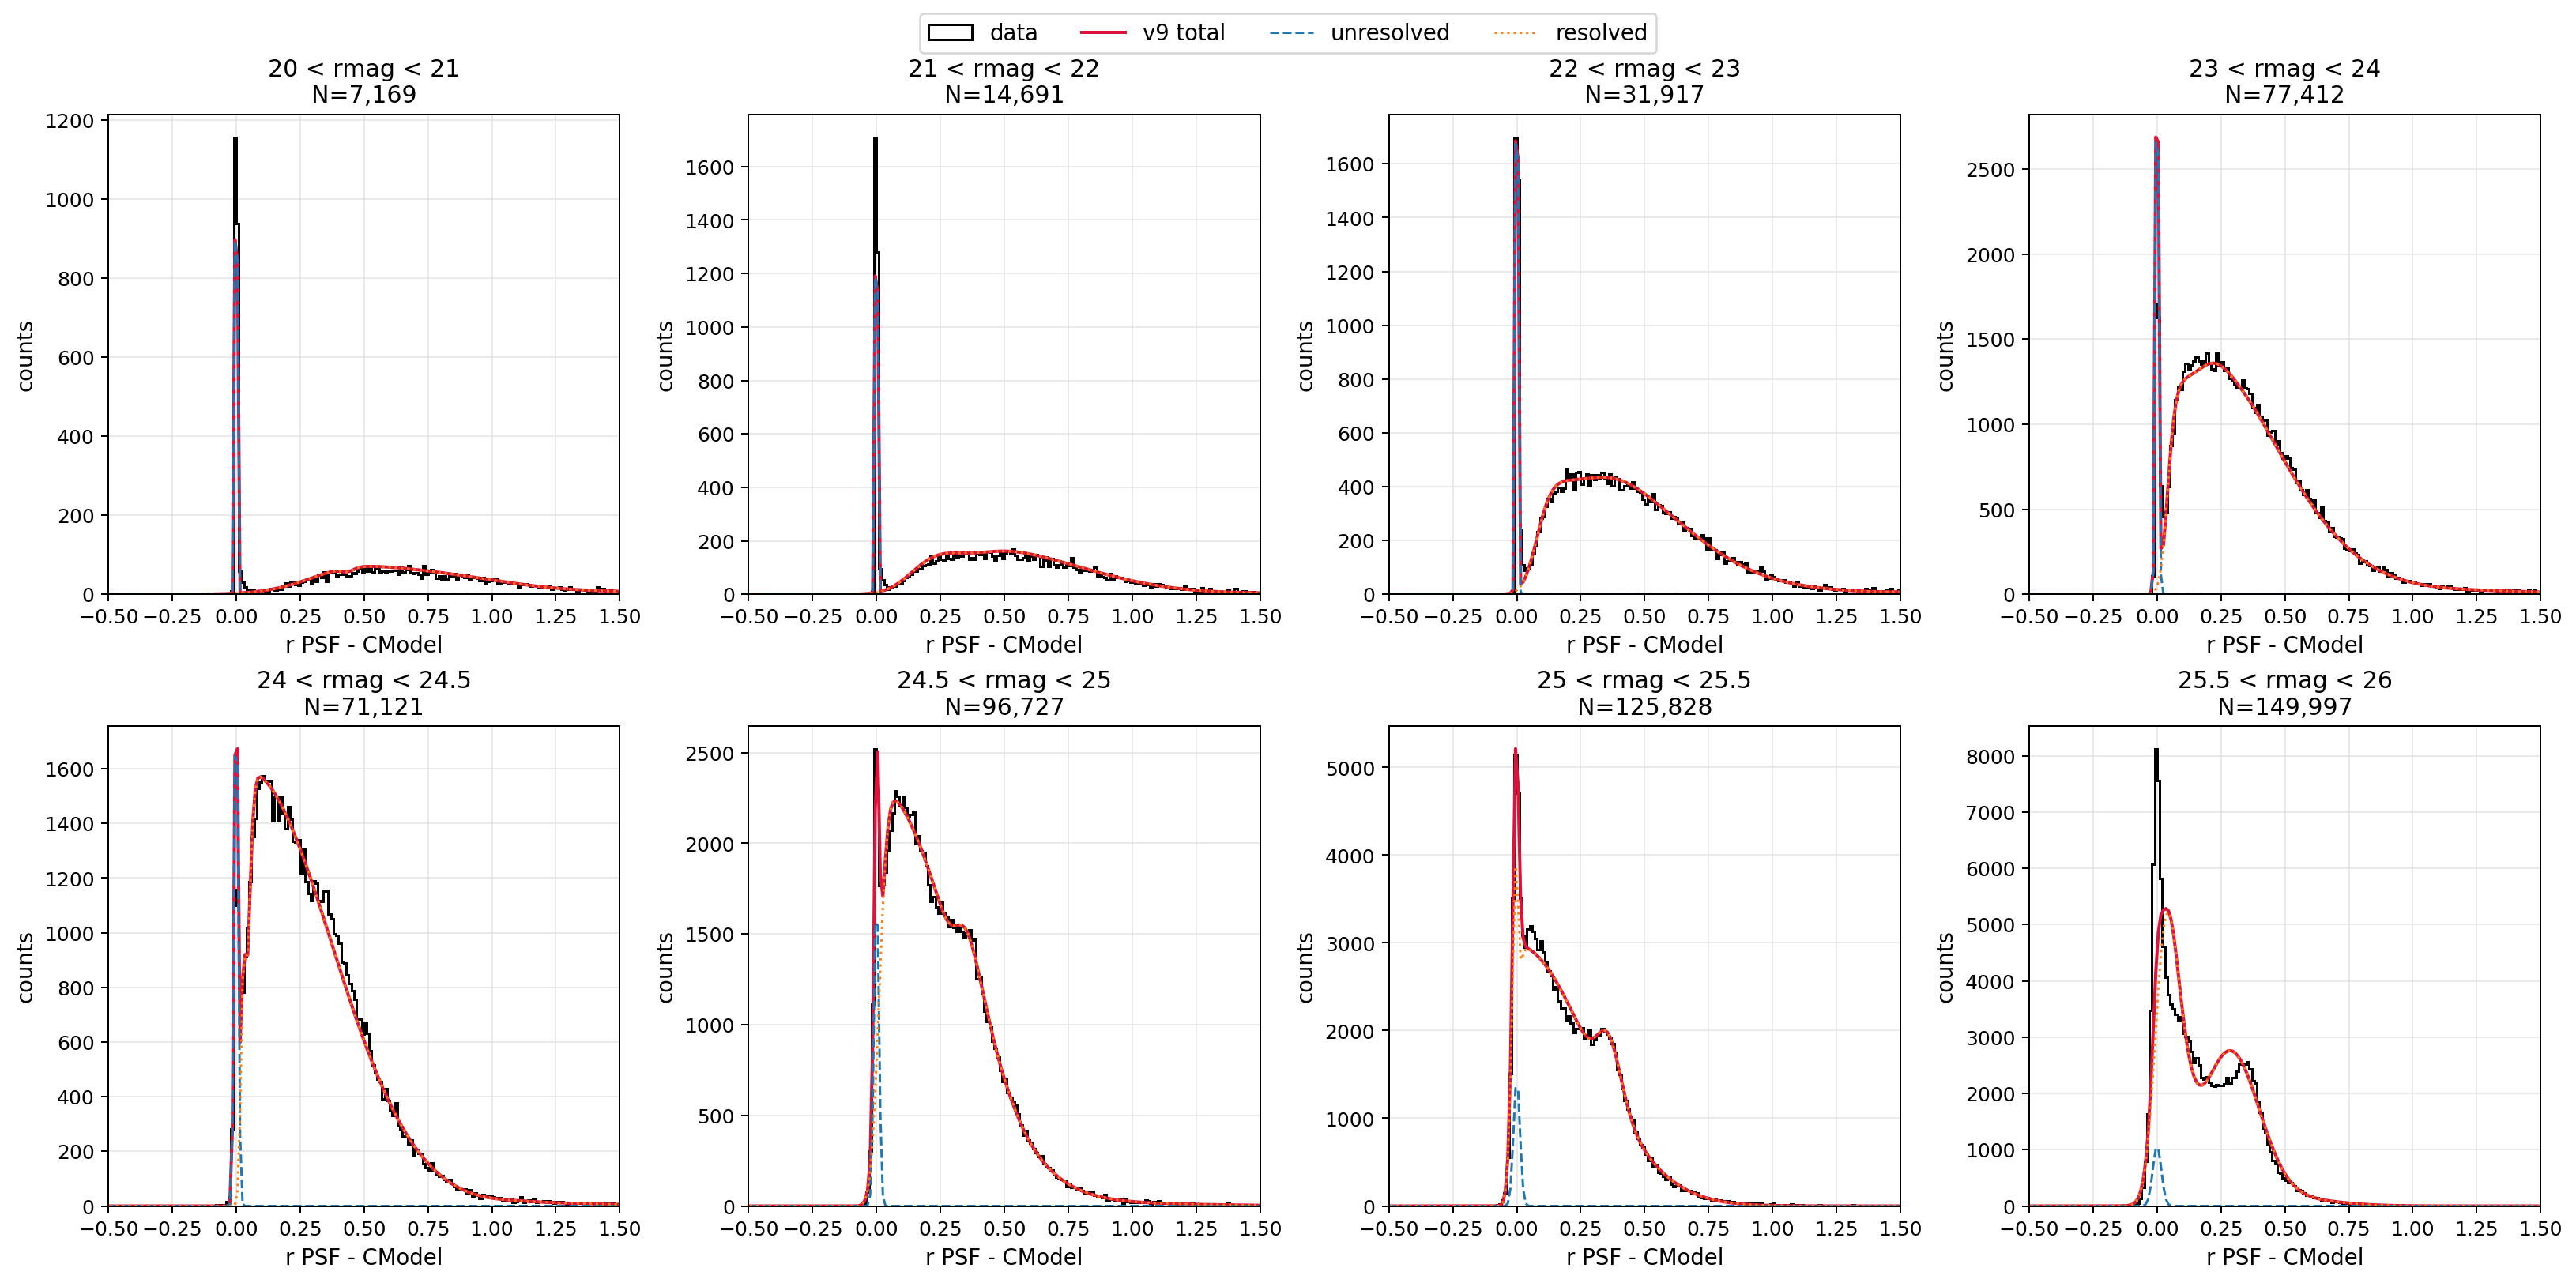
\includegraphics[width=\textwidth,height=0.72\textheight,keepaspectratio]{figures/section2_bayesian_method/fig2_2_cosmos_r_slice_fits_v9fit.png}
  \caption{Observed \(\Delta m\) histograms (black) and fitted mixture models (red) for the
    r-band in each CModel magnitude bin. The unresolved Gaussian component is shown as a blue
    dashed line and the resolved skew-normal components as orange dotted lines.}
  \label{fig:slice_fits}
\end{figure*}

\begin{figure*}
  \centering
  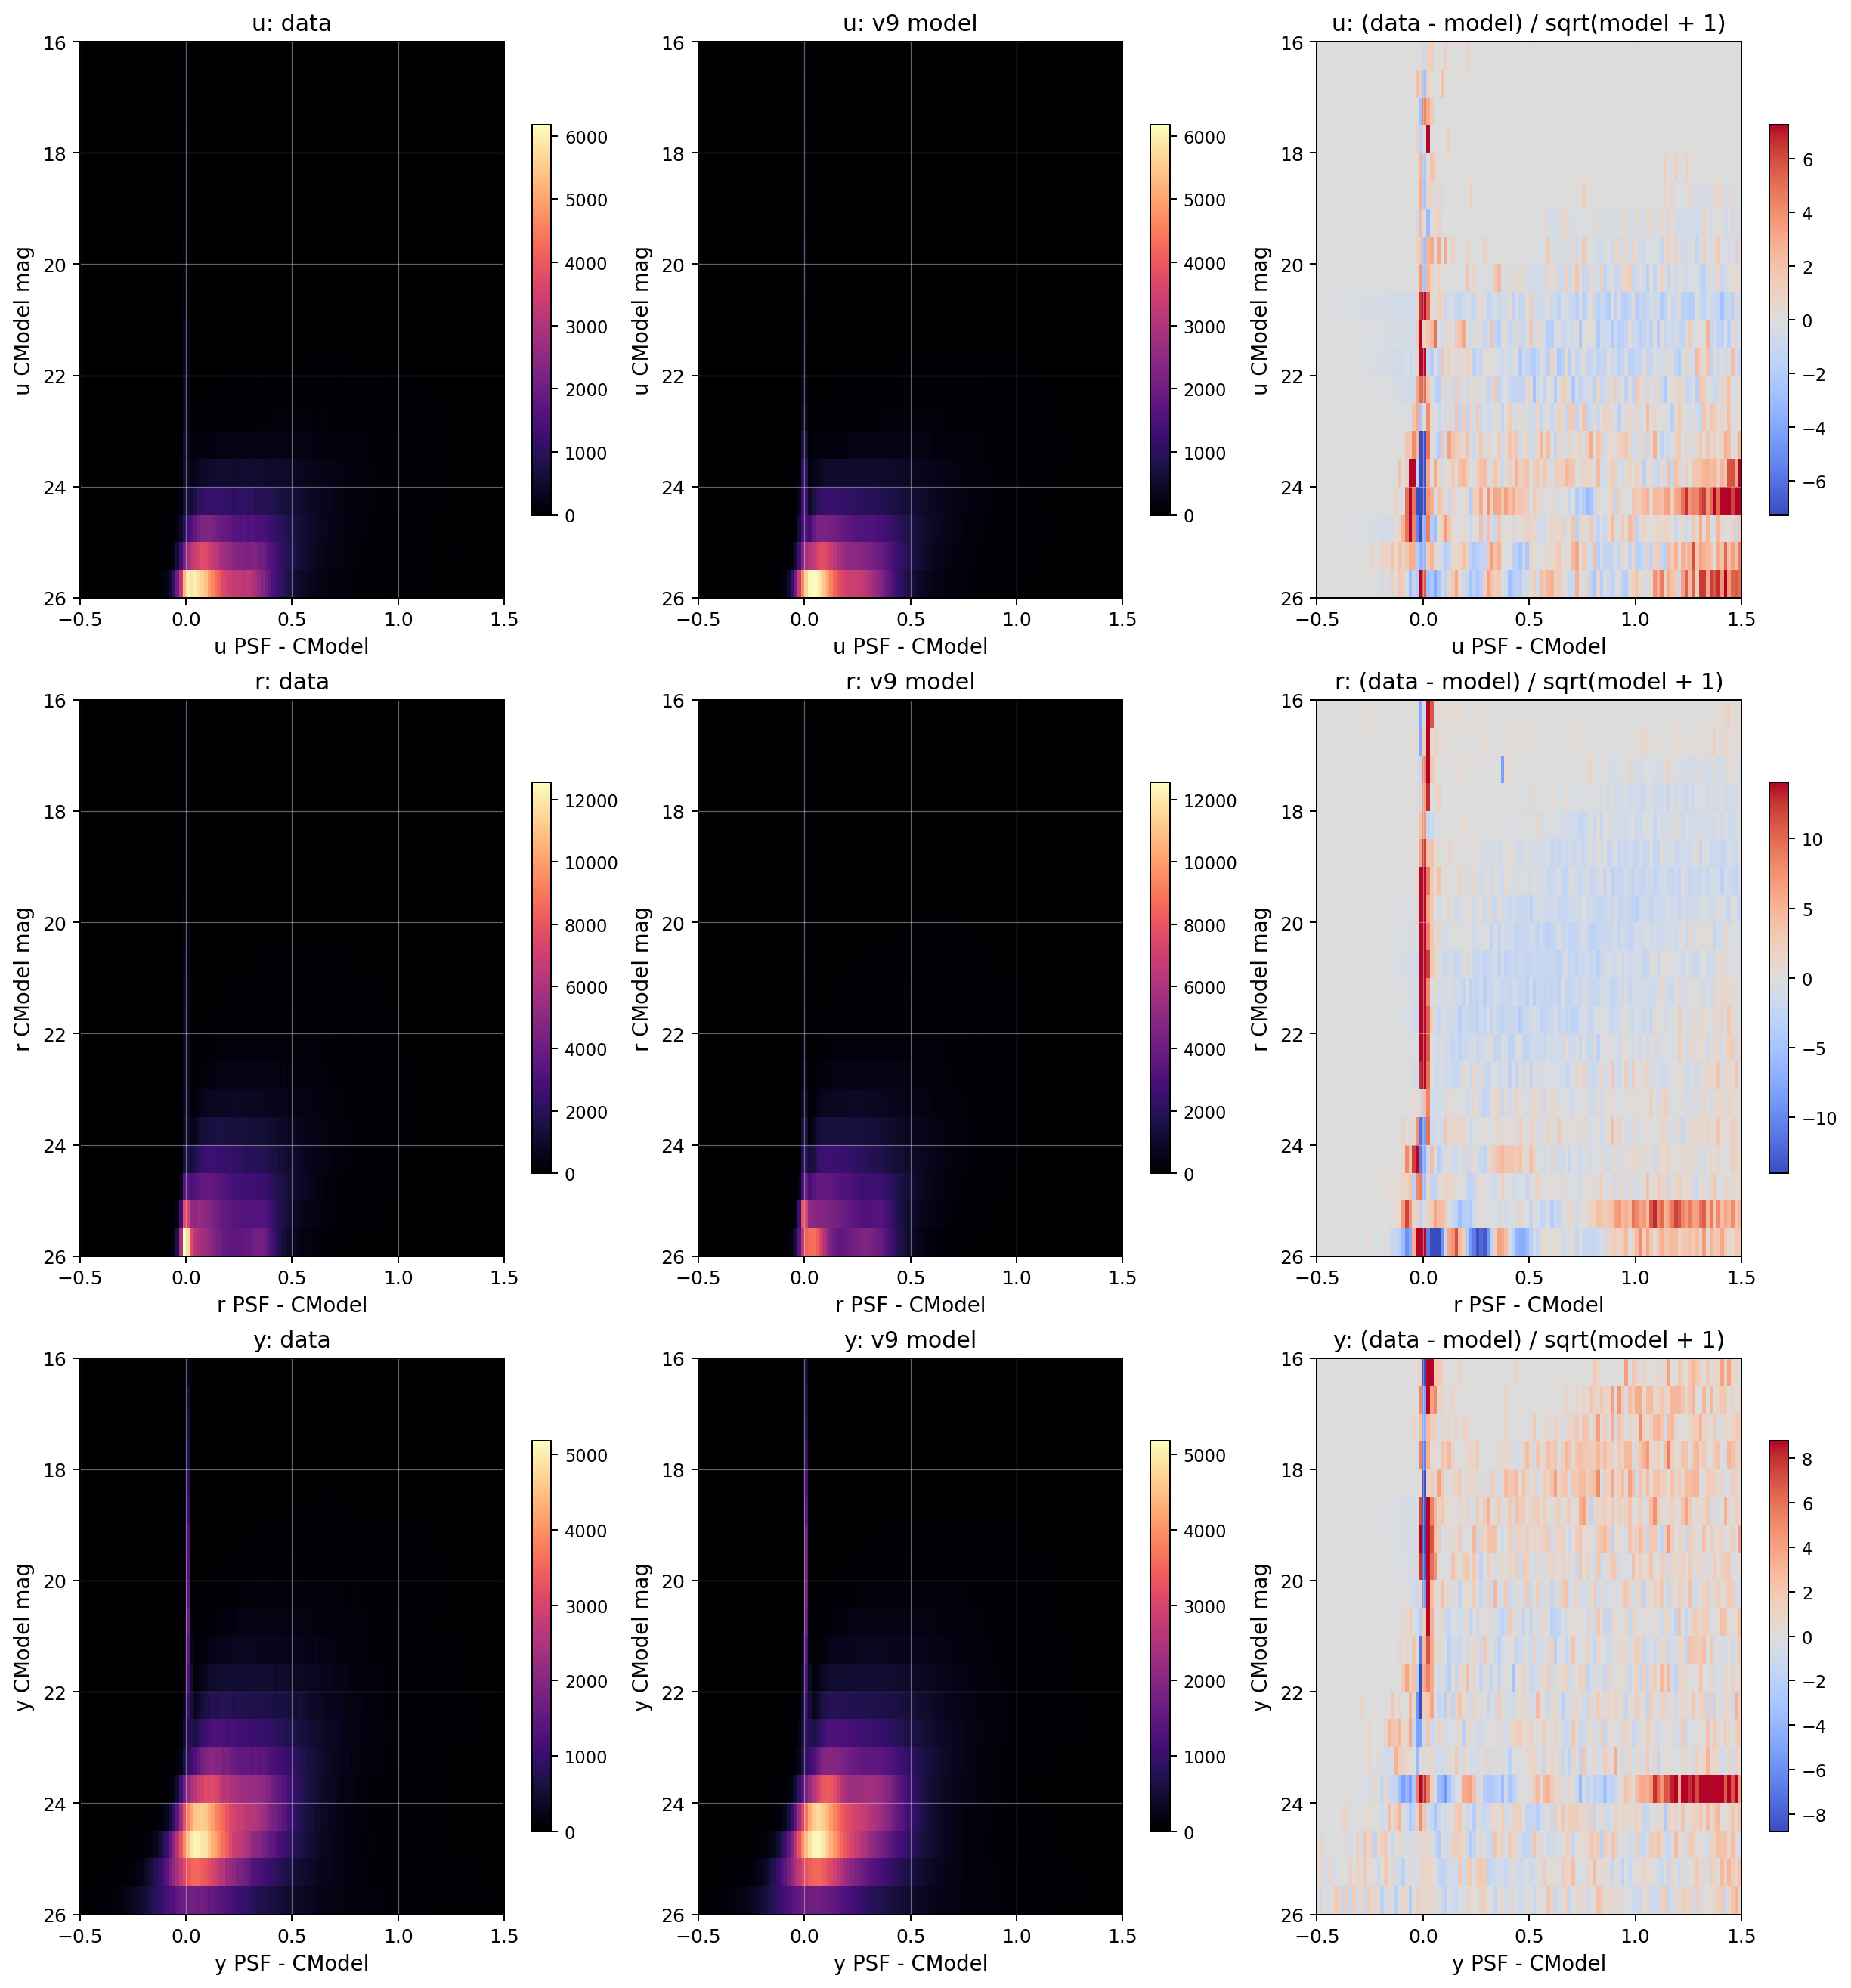
\includegraphics[width=\textwidth,height=0.82\textheight,keepaspectratio]{figures/section2_bayesian_method/fig2_3_cosmos_ury_model2d_residuals_v9fit.png}
  \caption{Two-dimensional comparison of the observed (left), modeled (center), and residual
    (right) source density in the \(\Delta m\) vs.\ \(m_{\mathrm{CModel}}\) plane. The small
    residuals demonstrate that the constrained mixture model provides an adequate description of
    the data across the full magnitude range.}
  \label{fig:model2d_residuals}
\end{figure*}


\subsection{The Performance of the \(\Delta m\) Mixture Model} 

Here we use HST labels to evaluate completeness and contamination for the stellar sample,
and to compare them to mixture model predictions. We focus on the stellar subsample and
the ``transition'' magnitude range: $24 < r < 24.5$: brighter than this limit the population
mixing is much smaller, while fainter than this limit the performance deteriorates rapidly
(especially for the stellar subsample).




 

% Bayes factor: BF(dm) = fG(dm) / fS(dm) 
% pS = fS(dm) / [fS(dm) + fG(dm)]

% pS = 1 / (1 + priorNGS * BF) 

% so 1/pS = 1 + prior * BF = 1 + prior * fG / fS
%    and   pS = 1 / (1 + prior NGS * fG / fS) 




\subsection{The Multi-band Case}

We expect classification to improve with more data but combining the information from different
bands is statistically complex problem... 
%\FloatBarrier

\section{Discussion and Conclusions}
\label{sec:discussion}

Reliable separation of unresolved and resolved sources is important for a
wide range of Rubin science applications.  Stellar-population studies require
samples with controlled galaxy contamination, while extragalactic analyses
require the complementary suppression of foreground stars.  These demands
become increasingly difficult to satisfy at faint magnitudes, where the
stellar and galaxy morphology distributions overlap and galaxies dominate the
source counts.  A continuous probabilistic description is therefore more
informative than a binary morphology flag because it retains the uncertainty
of each classification and allows independent measurements to be combined
before a catalog assignment is made
\citep{Henrion2011BayesianSG,Slater2020}.

XXXXXThe results in Section~\ref{sec:single-band-performance} show that most of the
improvement in the $r$-band ranking is obtained by modeling the full
magnitude-dependent morphology distributions.  For the 193,516 objects with a
finite $r$-band morphology measurement, the AUC increases from 0.871 for a
threshold sweep over the raw
$\Delta m_r=m_{{\rm PSF},r}-m_{{\rm CModel},r}$ measurement to 0.899 for the
morphology-only probabilistic score.  Including the source-count prior changes
the AUC to 0.901.  The comparatively small change in AUC does not make the
prior unimportant: AUC measures only the ordering of sources, whereas the
prior supplies the population odds required to interpret the morphology
likelihoods as posterior probabilities.  Its influence is greatest where the
morphology measurement is ambiguous and the two classes have very different
abundances \citep{Fawcett2006ROC}.

The fixed catalog assignment exposes the corresponding completeness--purity
trade-off.  At $16\leq r<24$, the probabilistic star-candidate sample has a
completeness of 0.878 and a purity of 0.975.  At $24\leq r<25$, its purity is
0.558, compared with 0.318 for the default Rubin
\texttt{extendedness} selection, while its completeness is 0.268, compared
with 0.582 for \texttt{extendedness}.  The probabilistic selection is thus
cleaner but less complete in this interval; it is not uniformly superior for
all scientific uses.  Analyses that prioritize rare-object discovery may
prefer higher completeness, whereas studies that are sensitive to galaxy
contamination may prefer the cleaner selection.  Reporting the continuous
$p_{\rm S}$ value preserves classification uncertainty in addition to the
adopted catalog assignment.  This class-specific reporting is particularly
important for the strongly imbalanced faint sample
\citep{SaitoRehmsmeier2015}.

At $25\leq r<26$, the adopted catalog assignment selects no star-like objects
in the evaluated sample.  The stellar completeness is consequently zero and
the purity of the empty star-candidate sample is undefined.  This result does
not imply that the field contains no stars.  Rather, the available morphology
information and the strongly galaxy-dominated source-count prior do not
produce posterior probabilities above the adopted assignment boundary.  The
continuous score still contains ranking information, but the present catalog
assignment is too conservative to define a useful faint stellar sample.  This
faint-end behavior is an important limitation rather than an improvement over
the Rubin baseline.

XXXXXThe multiband comparison leads to a similarly qualified conclusion.
Combining morphology measurements from additional bands improves the ranking
in the bright and intermediate intervals, but the gain is not monotonic with
the number of bands.  In the faintest interval, the $r$-only morphology score
slightly outperforms the six-band morphology score.  The color-augmented score
shown in Figure~\ref{fig:multiband-color-roc} improves the ranking relative to
the morphology-only curves within the evaluated sample, with its largest
displayed gain at the faint end.  Because the combined morphology-plus-color
quantity is used as a discriminative score rather than as a calibrated
likelihood ratio, it should be interpreted as a ranking statistic and not as
a posterior probability.  Likewise, the color distributions in
Figure~\ref{fig:color-distributions} describe the samples produced by the
classifier; because those colors contribute to the classification, that
figure is not an independent validation.  Previous work has similarly found
that multiband photometry can complement morphology, while also emphasizing
the dependence of performance on depth, labels, and survey conditions
\citep{Fadely2012MultiBandSG,Kim2015HybridSG,SevillaNoarbe2018DESY1}.

Several limitations determine how broadly the present measurements can be
generalized.  First, the validation is confined to the COSMOS field.  The
star-to-galaxy number ratio varies with Galactic coordinates, extinction,
depth, and catalog selection, so a prior inferred in COSMOS should not be
transferred unchanged across the Rubin footprint.  A spatially portable
version of the classifier could use a line-of-sight stellar-count prediction,
for example from TRILEGAL, together with an independently specified galaxy
count model \citep{Girardi2005TRILEGAL,DalTio2022TRILEGAL}.  TRILEGAL predicts
stellar counts rather than the galaxy-to-star ratio itself, and the stellar
and galaxy terms must be evaluated with consistent filters, extinction
conventions, magnitude bins, effective area, and catalog selections.

XXXXXSecond, 193,586 of the 269,606 selected Rubin sources are matched to the
COSMOS2020/FARMER reference catalog, a Rubin-side matching fraction of 0.718.
The reported metrics therefore characterize the matched validation sample,
not every selected Rubin source \citep{Weaver2022}.  The multiband comparisons
are further restricted to objects with finite values for every score included
in a given panel.  If matching failures or missing measurements depend on
class, magnitude, color, blending, or surface brightness, the evaluated sample
need not be representative of the full catalog.

Third, the external classifications are reference labels rather than
error-free physical truth.  High-resolution HST/ACS studies of COSMOS
demonstrate both the value and the magnitude dependence of morphology-based
reference samples \citep{Leauthaud2007COSMOSACS,Robin2007COSMOSStars}; we do
not assume that the COSMOS2020/FARMER labels used here are error free.
Independent checks with spectroscopic classifications and additional
high-resolution fields would help separate classifier errors from
reference-label errors and cosmic variance.

XXXXXFinally, the faint-end unresolved fraction is obtained by extrapolating a
smooth model from magnitude intervals in which the mixture components are
better separated.  The uncertainty of that extrapolation is not propagated
into the reported $p_{\rm S}$ values.  Future applications should propagate
uncertainties in the mixture parameters and population prior, and should test
sensitivity to depth, seeing, PSF modeling, blending, and crowding.  It is also
important to preserve the distinction between morphology and astrophysical
identity: $p_{\rm S}$ is formally the probability that a source belongs to the
unresolved morphological component.  Unresolved quasars and compact galaxies,
as well as resolved stellar systems, prevent this probability from being
universally identical to the probability that an object is physically a star.

XXXXXIn summary, modeling the full $\Delta m$ distribution extracts more ranking
information from the $r$-band morphology measurement than the binary Rubin
\texttt{extendedness} field and provides a continuous output that can be
combined with additional measurements.  In the matched COSMOS sample, the
probabilistic assignment produces a purer but less complete star-candidate
sample at $24\leq r<25$, while it becomes too conservative to select a useful
stellar sample at $25\leq r<26$.  Multiband morphology provides useful but
non-monotonic gains, and the color-augmented result is best regarded as a
ranking until it is probability-calibrated.  Extending the method across the
Rubin footprint will require field-dependent count priors, uncertainty
propagation, and validation in samples beyond the present COSMOS
complete-case data.

\bibliography{paper}{}
\bibliographystyle{aasjournalv7.1}
\end{document}

COMPILE WITH:
> latexmk -pdf paper.tex

 
%\input{methodZI}
%\input{methodBayes}
%\providecommand{\FloatBarrier}{\clearpage}

\section{Performance of the Bayesian Classifier}
\label{sec:performance}

\subsection{Validation Metrics}
\label{sec:validation-metrics}

We evaluate the classifiers using the matched COSMOS2020/FARMER reference
sample \citep{Weaver2022}.  The one-to-one match, constructed with a maximum
separation of $0.5\arcsec$, contains 193,586 objects: 8,788 reference-labeled
stars and 184,798 reference-labeled galaxies.  Throughout this section, $r$
denotes the Rubin $r$-band CModel magnitude.

The matched sample contains about 21 times more galaxies than stars, and the
imbalance is stronger at faint magnitudes.  A single accuracy value would
therefore be dominated by the much larger galaxy population.  We instead
evaluate the star-candidate and galaxy-candidate samples separately.  For a
target class $X$, where $X$ is either stars or galaxies, we define
completeness, purity, and contamination as

\begin{align}
    C_X &\equiv \frac{\mathrm{TP}_X}
                       {\mathrm{TP}_X+\mathrm{FN}_X},
    \label{eq:completeness}\\
    P_X &\equiv \frac{\mathrm{TP}_X}
                       {\mathrm{TP}_X+\mathrm{FP}_X},
    \label{eq:purity}\\
    f_{\mathrm{cont},X} &\equiv 1-P_X
      =\frac{\mathrm{FP}_X}{\mathrm{TP}_X+\mathrm{FP}_X}.
    \label{eq:contamination}
\end{align}

Completeness is the fraction of reference objects of class $X$ that are
recovered, whereas purity is the fraction of the selected sample that belongs
to class $X$ according to the reference labels.  Purity is particularly
important for the imbalanced faint sample because even a modest false-positive
rate can produce substantial contamination \citep{SaitoRehmsmeier2015}.

For a receiver operating characteristic (ROC) curve, the false-positive rate
for target class $X$ is

\begin{equation}
    \mathrm{FPR}_X \equiv
    \frac{\mathrm{FP}_X}{\mathrm{FP}_X+\mathrm{TN}_X}.
    \label{eq:false-positive-rate}
\end{equation}

Its denominator contains all reference members of the opposite class and
therefore differs from the denominator of contamination.  The true-positive
rate on the ROC curve is equal to $C_X$.  The area under the ROC curve (AUC)
summarizes how well a continuous score orders the two classes
\citep{Fawcett2006ROC}.

\subsection{Single-band Morphology Performance}
\label{sec:single-band-performance}

We use the continuous $r$-band scores to compare how well the two reference
classes are separated, and we use the fixed catalog rules to measure the
completeness and purity of the selected samples.  Every probabilistic catalog
classification in this section uses $p_{{\rm S},r}\geq0.5$ for a star-like
assignment.  The Rubin comparison uses its default boundary,
$\Delta m_r\leq0.016\,\mathrm{mag}$.

\begin{figure*}[!t]
    \centering
    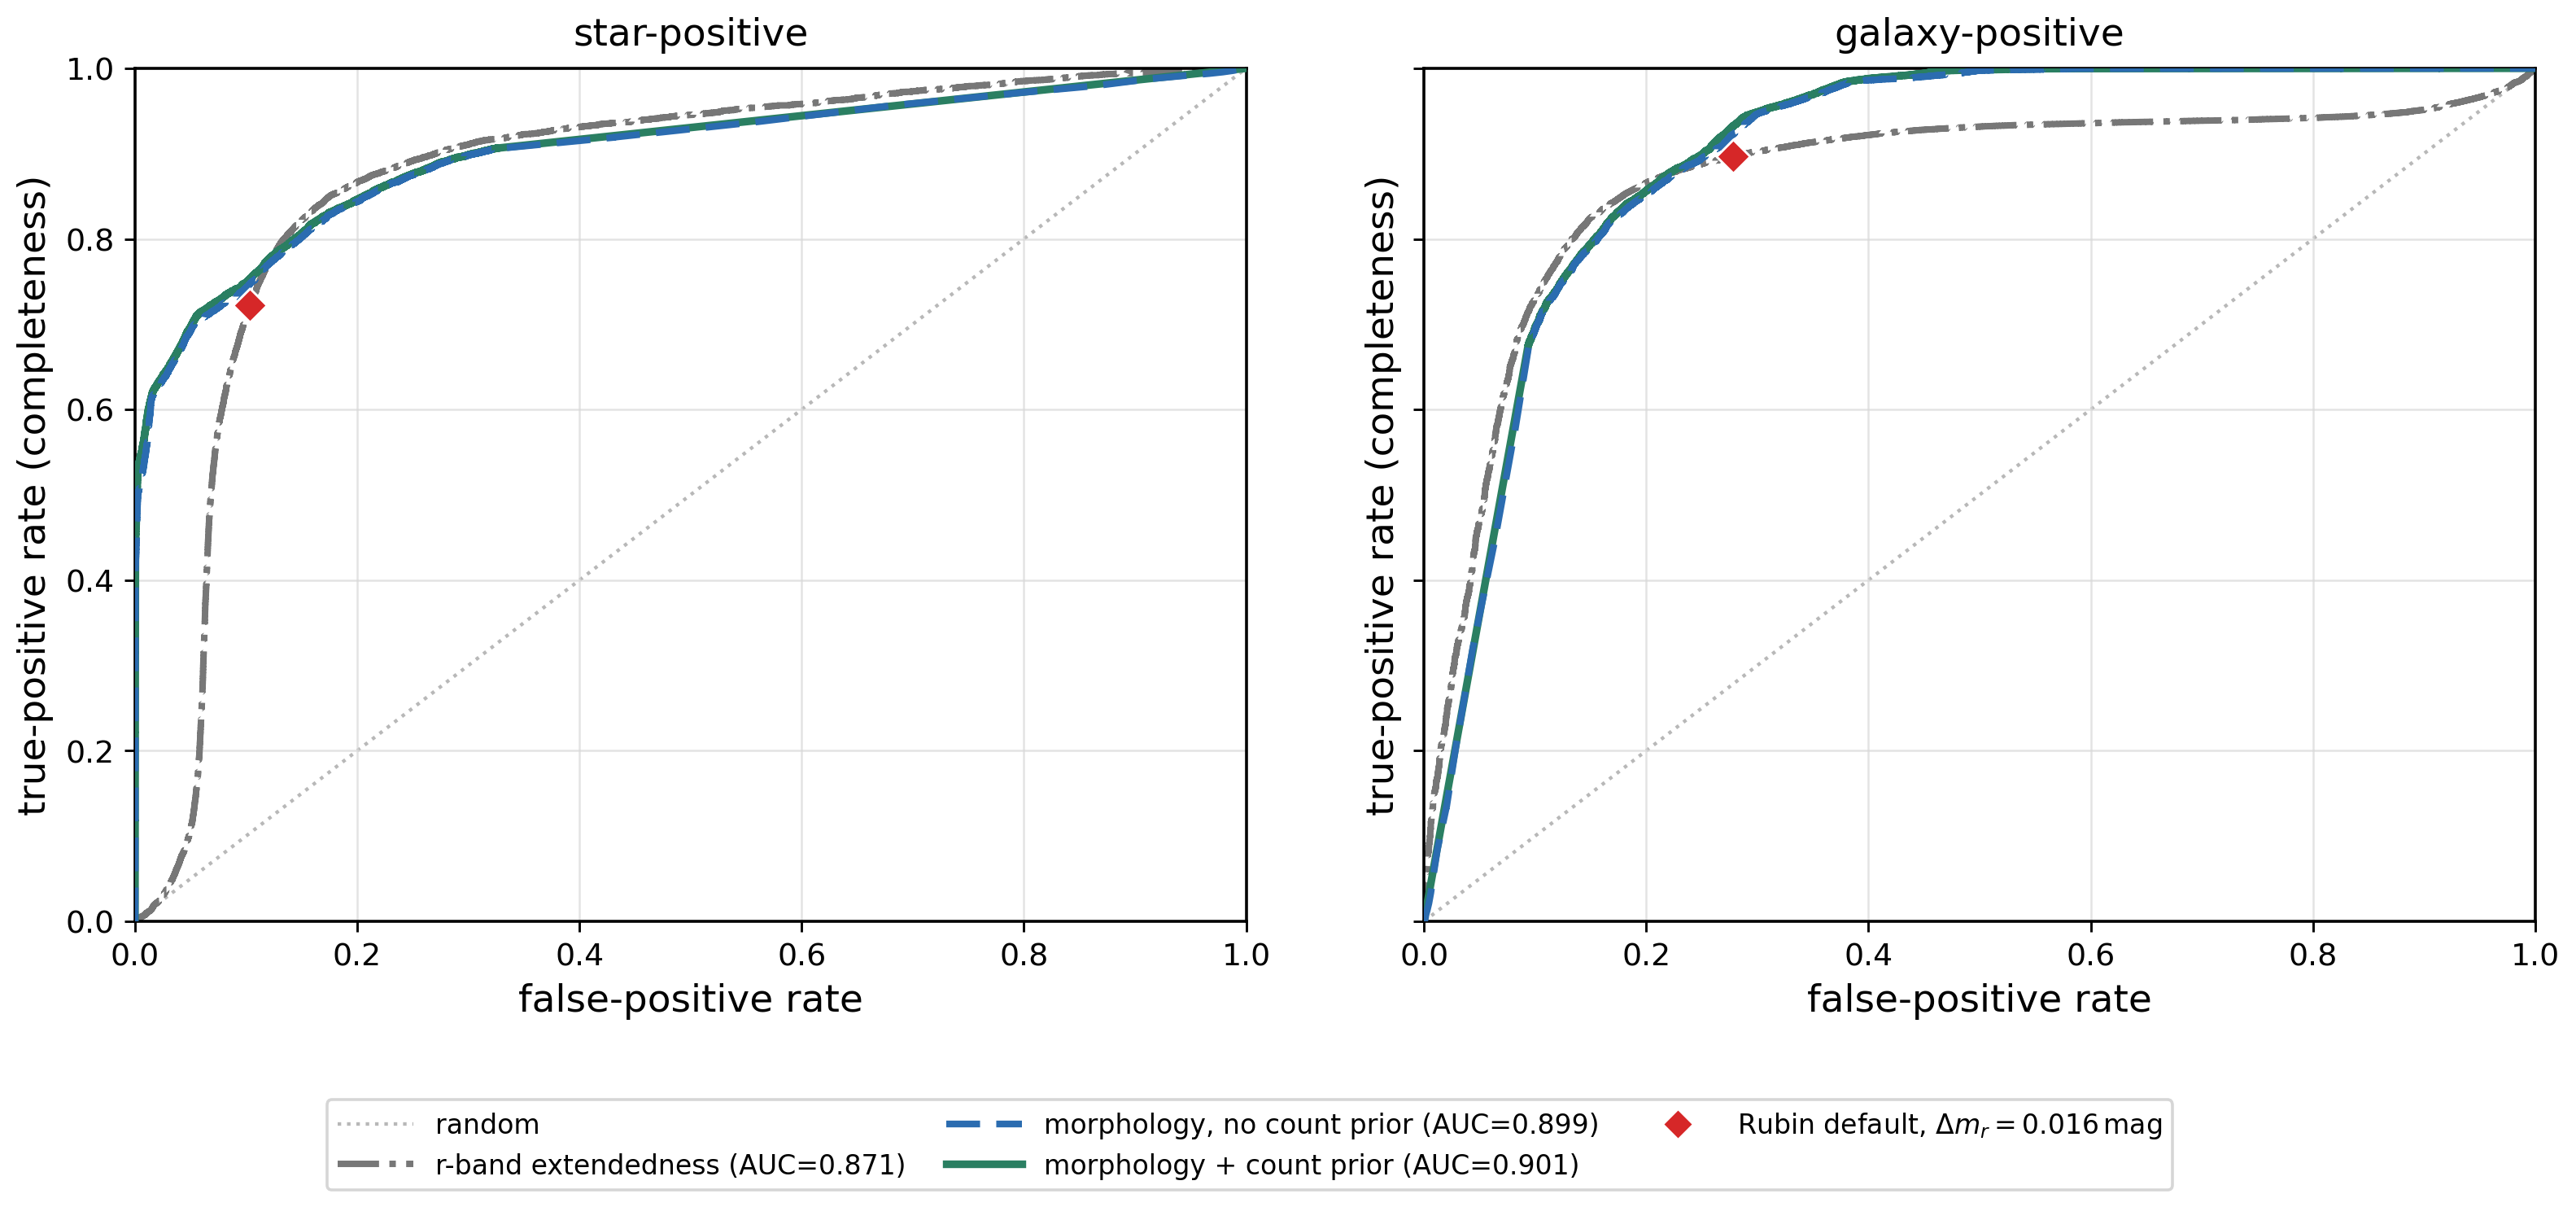
\includegraphics[width=\textwidth]{fig09_morphology_only_roc.png}
    \caption{Performance of the continuous $r$-band morphology scores for the
    $0.5\arcsec$ COSMOS validation sample.  The left and right panels treat stars
    and galaxies as the target class, respectively.  The gray dash-dotted curve
    uses raw $\Delta m_r$, the blue curve uses the fitted morphology distributions
    without the source-count prior, and the green curve includes the prior.  The
    red diamond marks the fixed Rubin \texttt{extendedness} assignment at
    $\Delta m_r=0.016\,\mathrm{mag}$, and the black circle marks the fixed
    probabilistic assignment at $p_{{\rm S},r}=0.5$.  Values in parentheses give
    the AUC of each continuous score.}
    \label{fig:rband-roc}
\end{figure*}

\subsubsection{Ranking of the Continuous Scores}
\label{sec:rband-ranking}

Figure~\ref{fig:rband-roc} compares three continuous $r$-band morphology
scores.  The first is the measured quantity

\begin{equation}
    \Delta m_r=m_{{\rm PSF},r}-m_{{\rm CModel},r},
    \label{eq:delta-m-r}
\end{equation}

which underlies the Rubin \texttt{extendedness} classification.  The gray
curve therefore measures the discriminatory information in the raw
$\Delta m_r$ values.  The fixed Rubin catalog classification is shown
separately by the red diamond at $\Delta m_r=0.016\,\mathrm{mag}$.  Likewise,
the fixed probabilistic classification at $p_{{\rm S},r}=0.5$ is marked on the
prior-informed score by the black circle.

The blue and green curves use the fitted class-conditional morphology
distributions described in Section~\ref{sec:mixture-model}.  The blue score
omits the magnitude-dependent source-count prior, whereas the green score
includes the prior from Section~\ref{sec:sg-priors}.  All three scores are
evaluated on the same 193,516 objects with finite $r$-band morphology
measurements.

The AUC is 0.871 for raw $\Delta m_r$, 0.899 for the morphology model without
the count prior, and 0.901 after the prior is included.  The modeled
class-conditional distributions therefore improve the overall ordering, while
the count prior changes the global AUC only slightly.  The ROC curves cross:
raw $\Delta m_r$ lies above the modeled scores over parts of the displayed
false-positive-rate range, while the modeled scores perform better elsewhere.
The higher AUC therefore describes an improvement averaged over the full
curve, not uniform dominance at every operating region.

\subsubsection{Completeness and Purity of the Fixed Catalog Samples}
\label{sec:rband-catalog-performance}

Figure~\ref{fig:rband-fixed-performance} compares the samples produced by the
fixed $p_{{\rm S},r}=0.5$ and Rubin \texttt{extendedness} rules in three
magnitude intervals.  The unresolved-selected and resolved-selected samples
are treated as star-candidate and galaxy-candidate samples, respectively.  We
show completeness and purity; contamination is simply $1-P_X$.

At $16\leq r<24$, the probabilistic star-candidate sample has completeness
0.878 and purity 0.975, similar to the Rubin selection in this interval.  At
$24\leq r<25$, the two methods make a different trade-off: the probabilistic
selection increases stellar purity from 0.318 to 0.558, while stellar
completeness decreases from 0.582 to 0.268.

At $25\leq r<26$, no evaluated object satisfies $p_{{\rm S},r}\geq0.5$.
Stellar completeness is therefore zero, and stellar purity is undefined
because the selected sample is empty.  Thus, the fixed prior-informed
$r$-band rule does not produce a usable star-candidate sample in the faintest
interval.  The galaxy-candidate sample remains nearly complete and highly
pure, but these values are aided by the overwhelming numerical dominance of
galaxies and do not imply comparable recovery of the rare stellar population.

\begin{figure*}[!t]
    \centering
    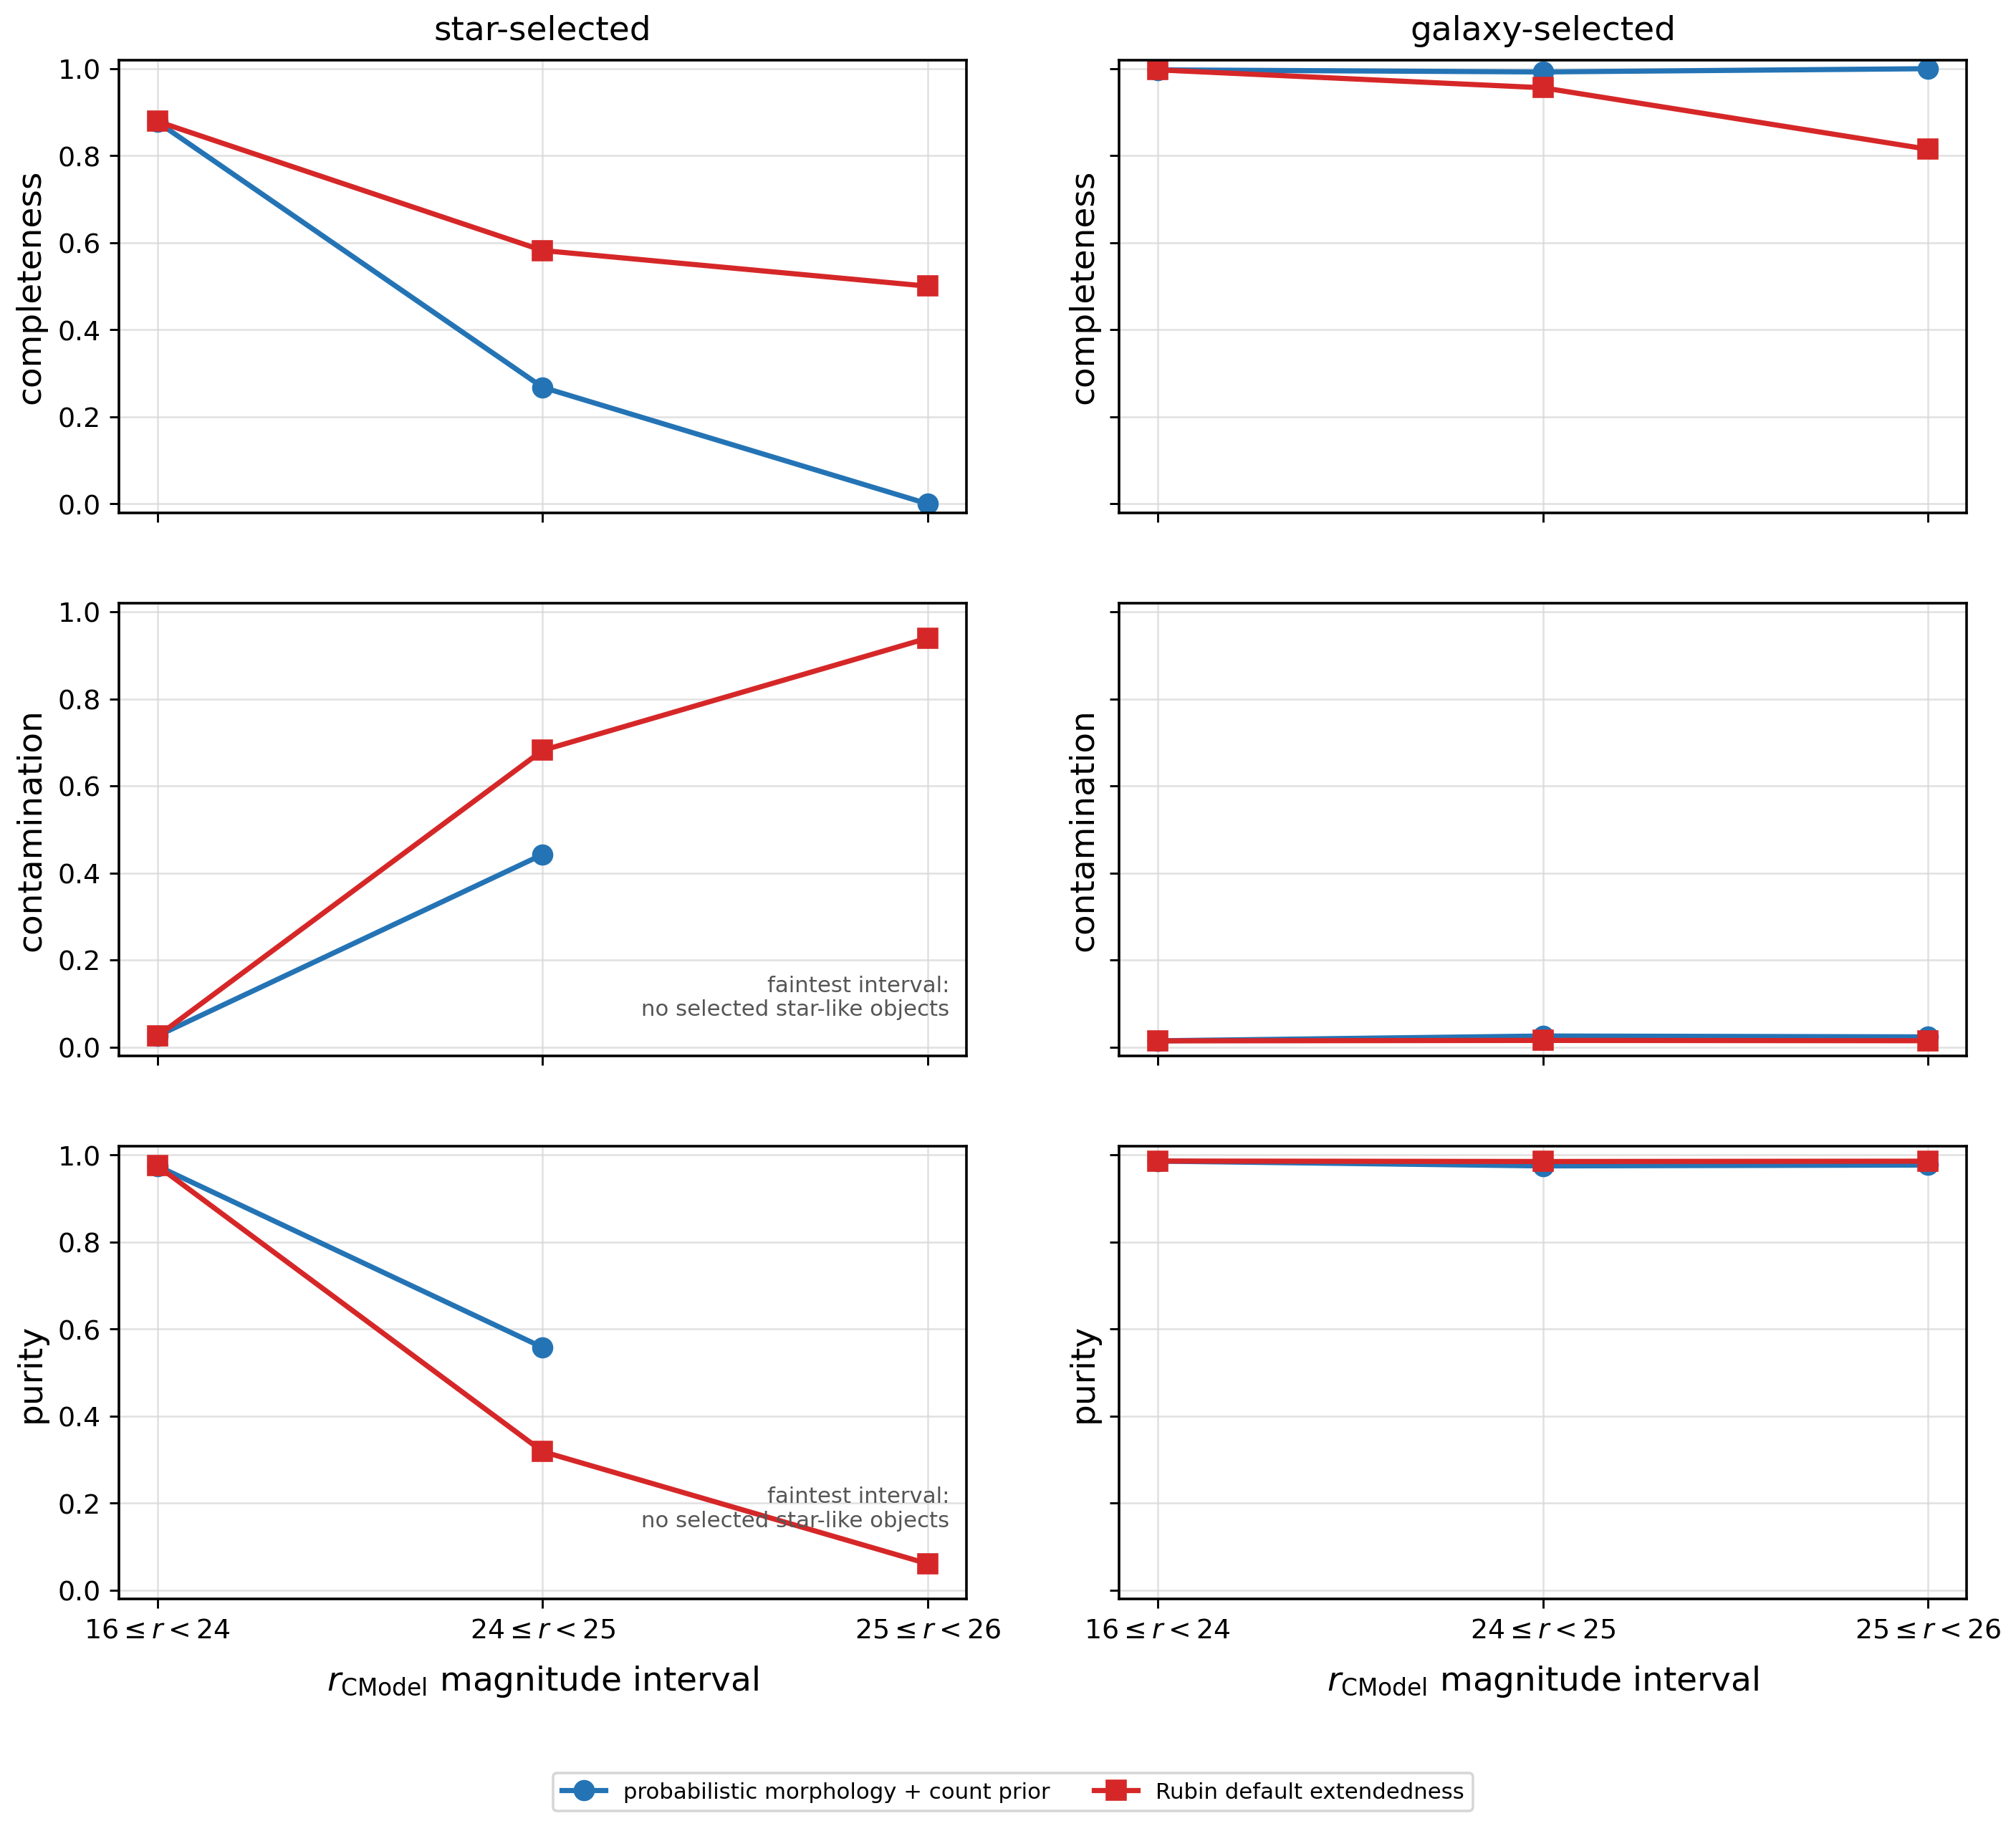
\includegraphics[width=\textwidth]{fig10_single_band_performance.png}
    \caption{Completeness (top row) and purity (bottom row) of the
    star-candidate sample (left column) and galaxy-candidate sample (right column)
    in three $r$-band magnitude intervals.  Horizontally offset markers compare
    the fixed $p_{{\rm S},r}=0.5$ assignment with the default Rubin
    \texttt{extendedness} assignment; the magnitude intervals are not connected
    by lines.  Error bars show 68\% Wilson binomial intervals, and annotations give
    the number of selected objects.  At $25\leq r<26$, the probabilistic method
    selects no star-like objects, so stellar completeness is zero and stellar
    purity is undefined and is not plotted.}
    \label{fig:rband-fixed-performance}
\end{figure*}

\subsection{Multiband Morphology and Color Information}
\label{sec:multiband-color}

Morphology and broadband colors provide complementary information for
star--galaxy separation
\citep{Fadely2012MultiBandSG,Kim2015HybridSG,SevillaNoarbe2018DESY1}.
Figure~\ref{fig:multiband-color-roc} compares scores based on $r$-band
morphology, $gri$ morphology, all six $ugrizy$ morphology measurements, and a
combined morphology-plus-color score.  The band-level morphology information
is combined before the magnitude-dependent source-count prior is applied.
Within each magnitude interval, all curves use the same complete-case sample.

\begin{figure*}[!t]
    \centering
    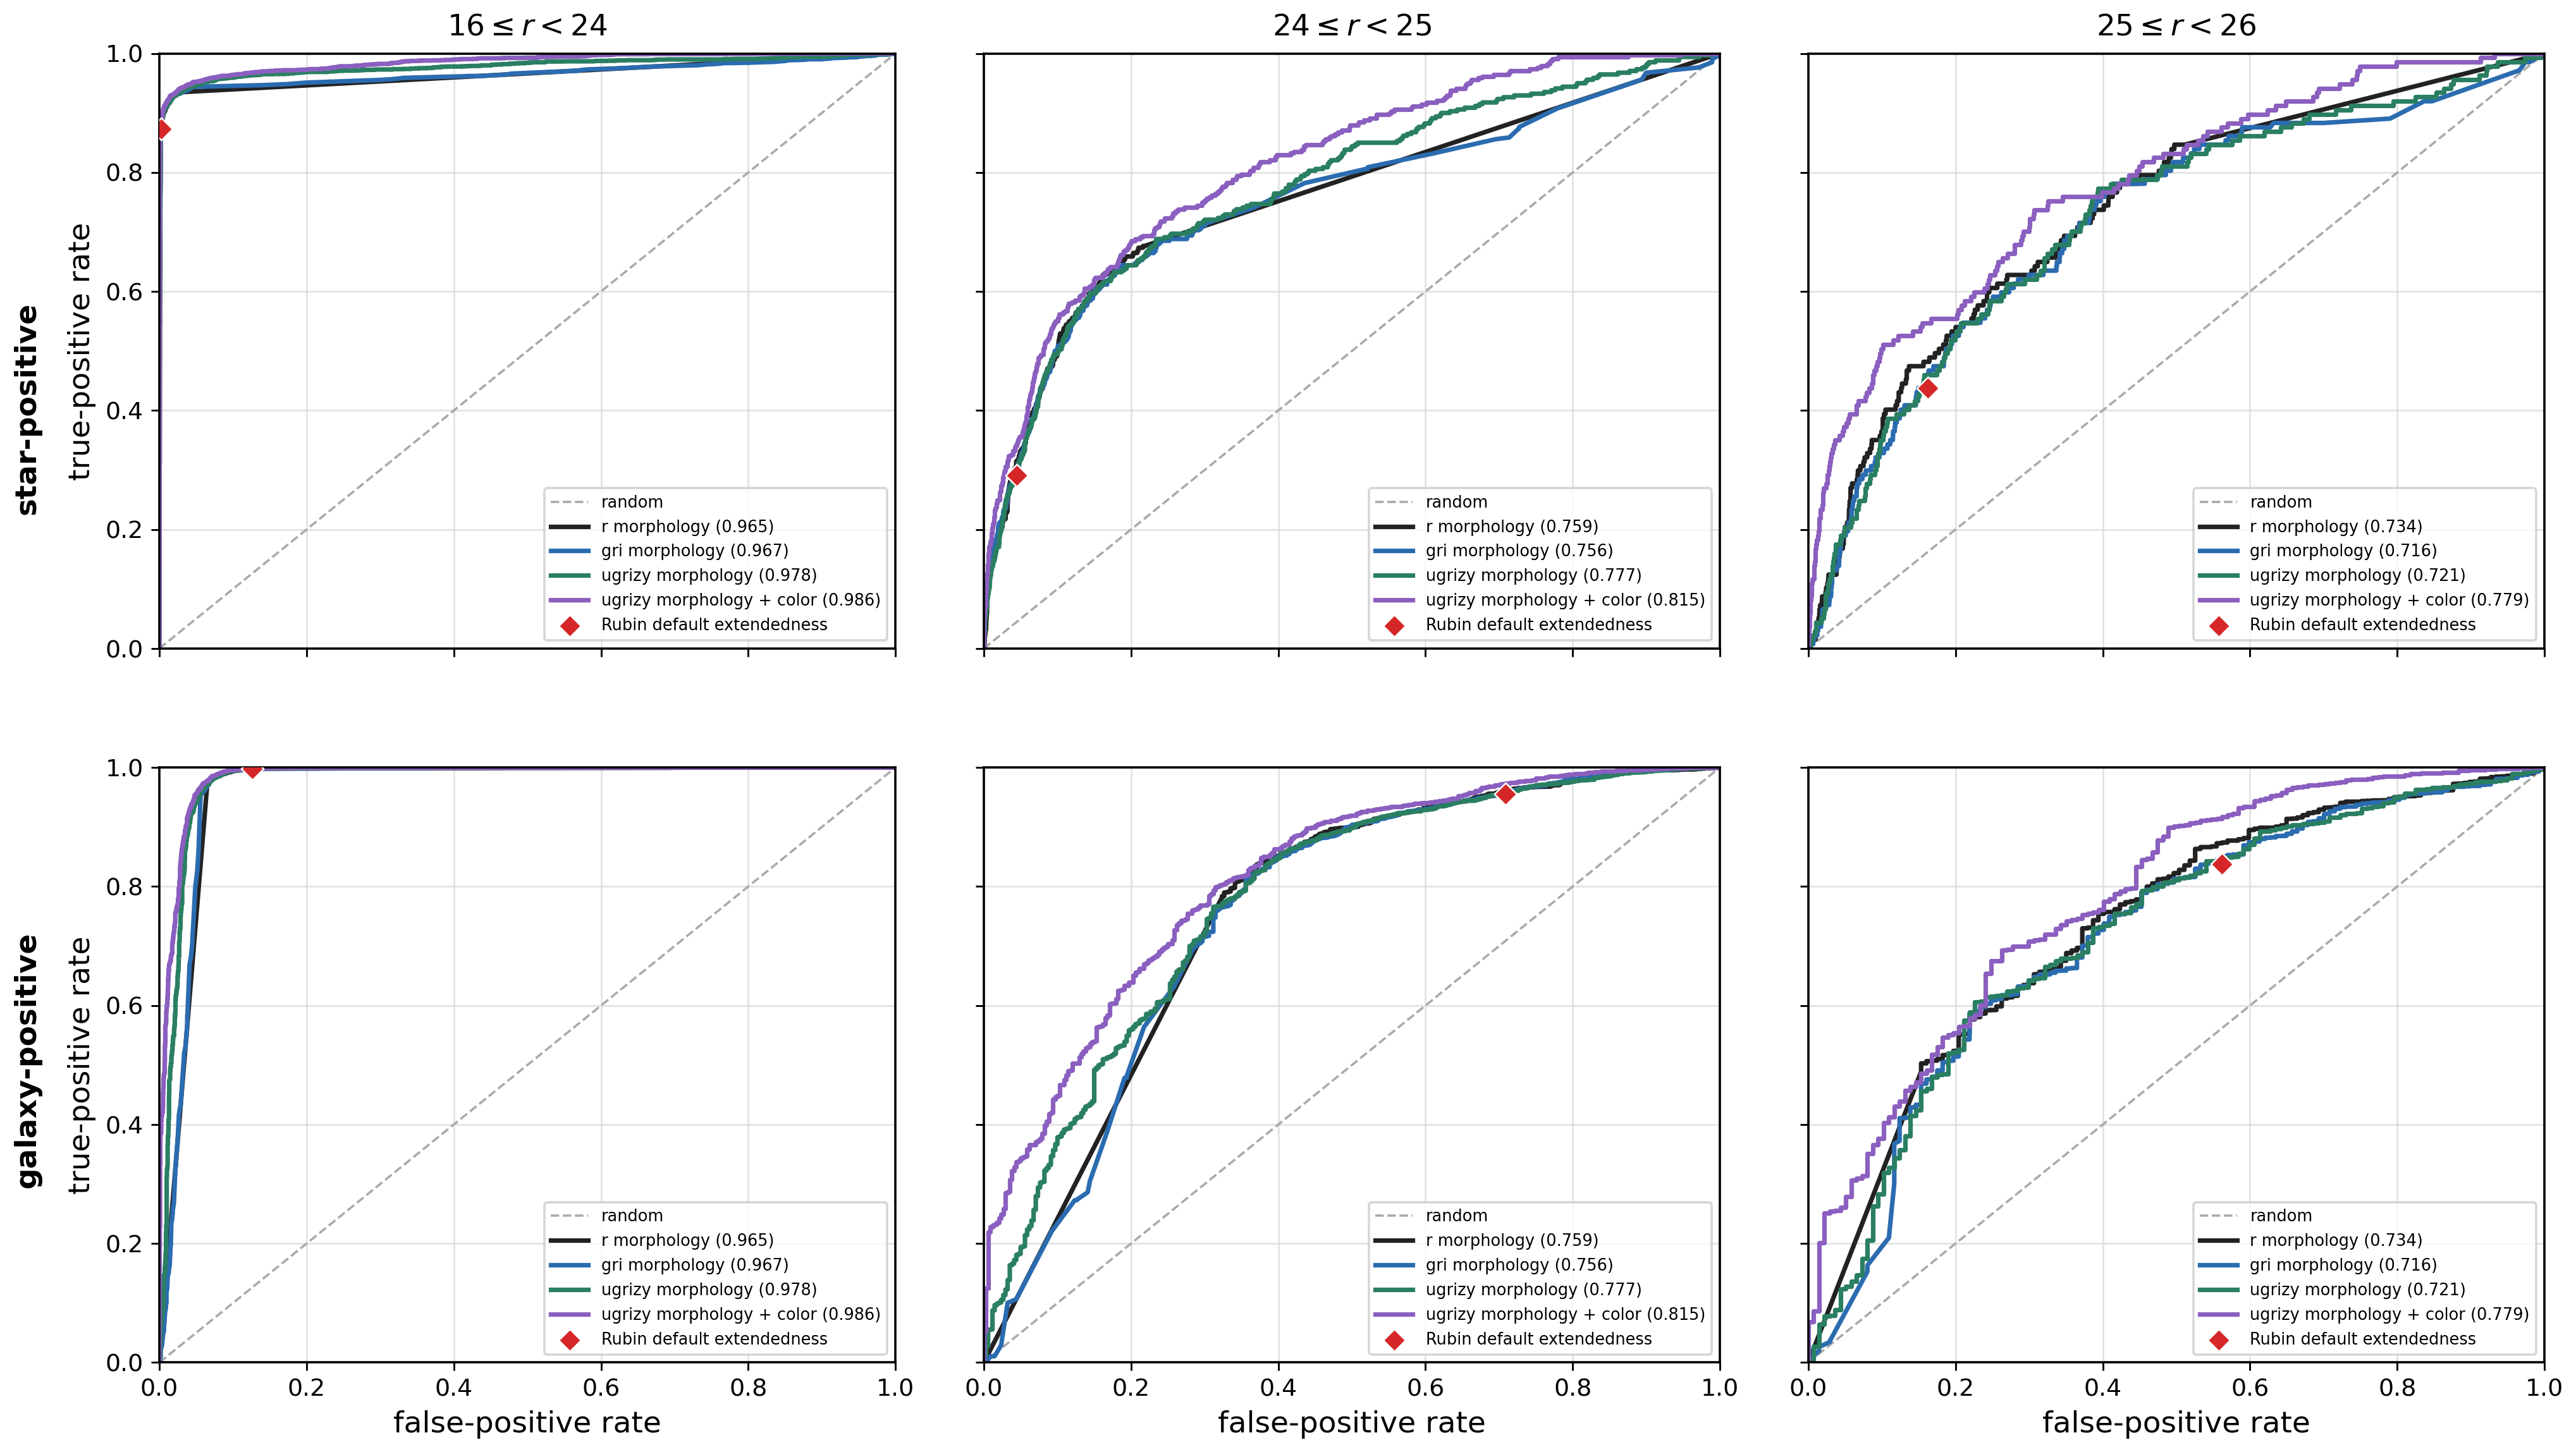
\includegraphics[width=\textwidth]{fig11_multiband_color_roc.png}
    \caption{Ranking performance obtained from multiband morphology and color
    information.  The top and bottom rows treat stars and galaxies as the target
    class, respectively, and the columns show three $r$-band magnitude intervals.
    Curves compare morphology information from the $r$, $gri$, and $ugrizy$ bands
    with the combined $ugrizy$ morphology-plus-color score.  Every panel uses a
    common complete-case sample.  The red diamond marks the default Rubin
    $r$-band \texttt{extendedness} assignment at
    $\Delta m_r=0.016\,\mathrm{mag}$.  Values in parentheses give the AUC.}
    \label{fig:multiband-color-roc}
\end{figure*}

The combined score supplements the $ugrizy$ morphology information with the
output of a Random Forest classifier based on the five adjacent colors
$(u-g,g-r,r-i,i-z,z-y)$ \citep{Breiman2001RandomForests}.  Figure~\ref{fig:multiband-color-roc}
uses this output together with the multiband morphology score as a continuous
classifier score.

% Before submission, verify from the implementation that the Random Forest
% values used here are held-out or out-of-fold predictions and confirm the
% exact rule used to combine the color and morphology scores.

For the star-positive comparison, the $ugrizy$ morphology AUC is 0.978,
0.777, and 0.721 in the three magnitude intervals, compared with 0.965,
0.759, and 0.734 for $r$-band morphology alone.  The six-band morphology score
therefore gives modest gains in the first two intervals, while the $r$-only
score is slightly higher in the faintest interval.  The $gri$ score is also
slightly below the $r$-only result in the two faint intervals.  These
comparisons show that the contribution of an additional morphology band
depends on the useful depth of its measurements, rather than simply on the
number of bands included.

Including the color score changes the $ugrizy$ morphology AUC from 0.978 to
0.986, from 0.777 to 0.815, and from 0.721 to 0.779.  The corresponding
increments are $+0.008$, $+0.038$, and $+0.058$, so the additional separation
provided by color becomes progressively larger across the three displayed
magnitude intervals.  The top row of
Figure~\ref{fig:multiband-color-roc} gives the completeness of reference stars
as galaxies are admitted into the star-selected sample, while the bottom row
gives the completeness of reference galaxies as stars are admitted into the
galaxy-selected sample.  The two rows therefore expose the trade-off relevant
to each selected class directly.

\subsection{Color Distributions of the Classifier-selected Samples}
\label{sec:classifier-selected-colors}

Figure~\ref{fig:color-distributions} shows how the unresolved and resolved
assignments from the combined $ugrizy$ morphology-plus-color classifier are
distributed in four two-dimensional color projections.  This provides a
direct view of the color-space partition produced by the final classifier.

\begin{figure*}[!t]
    \centering
    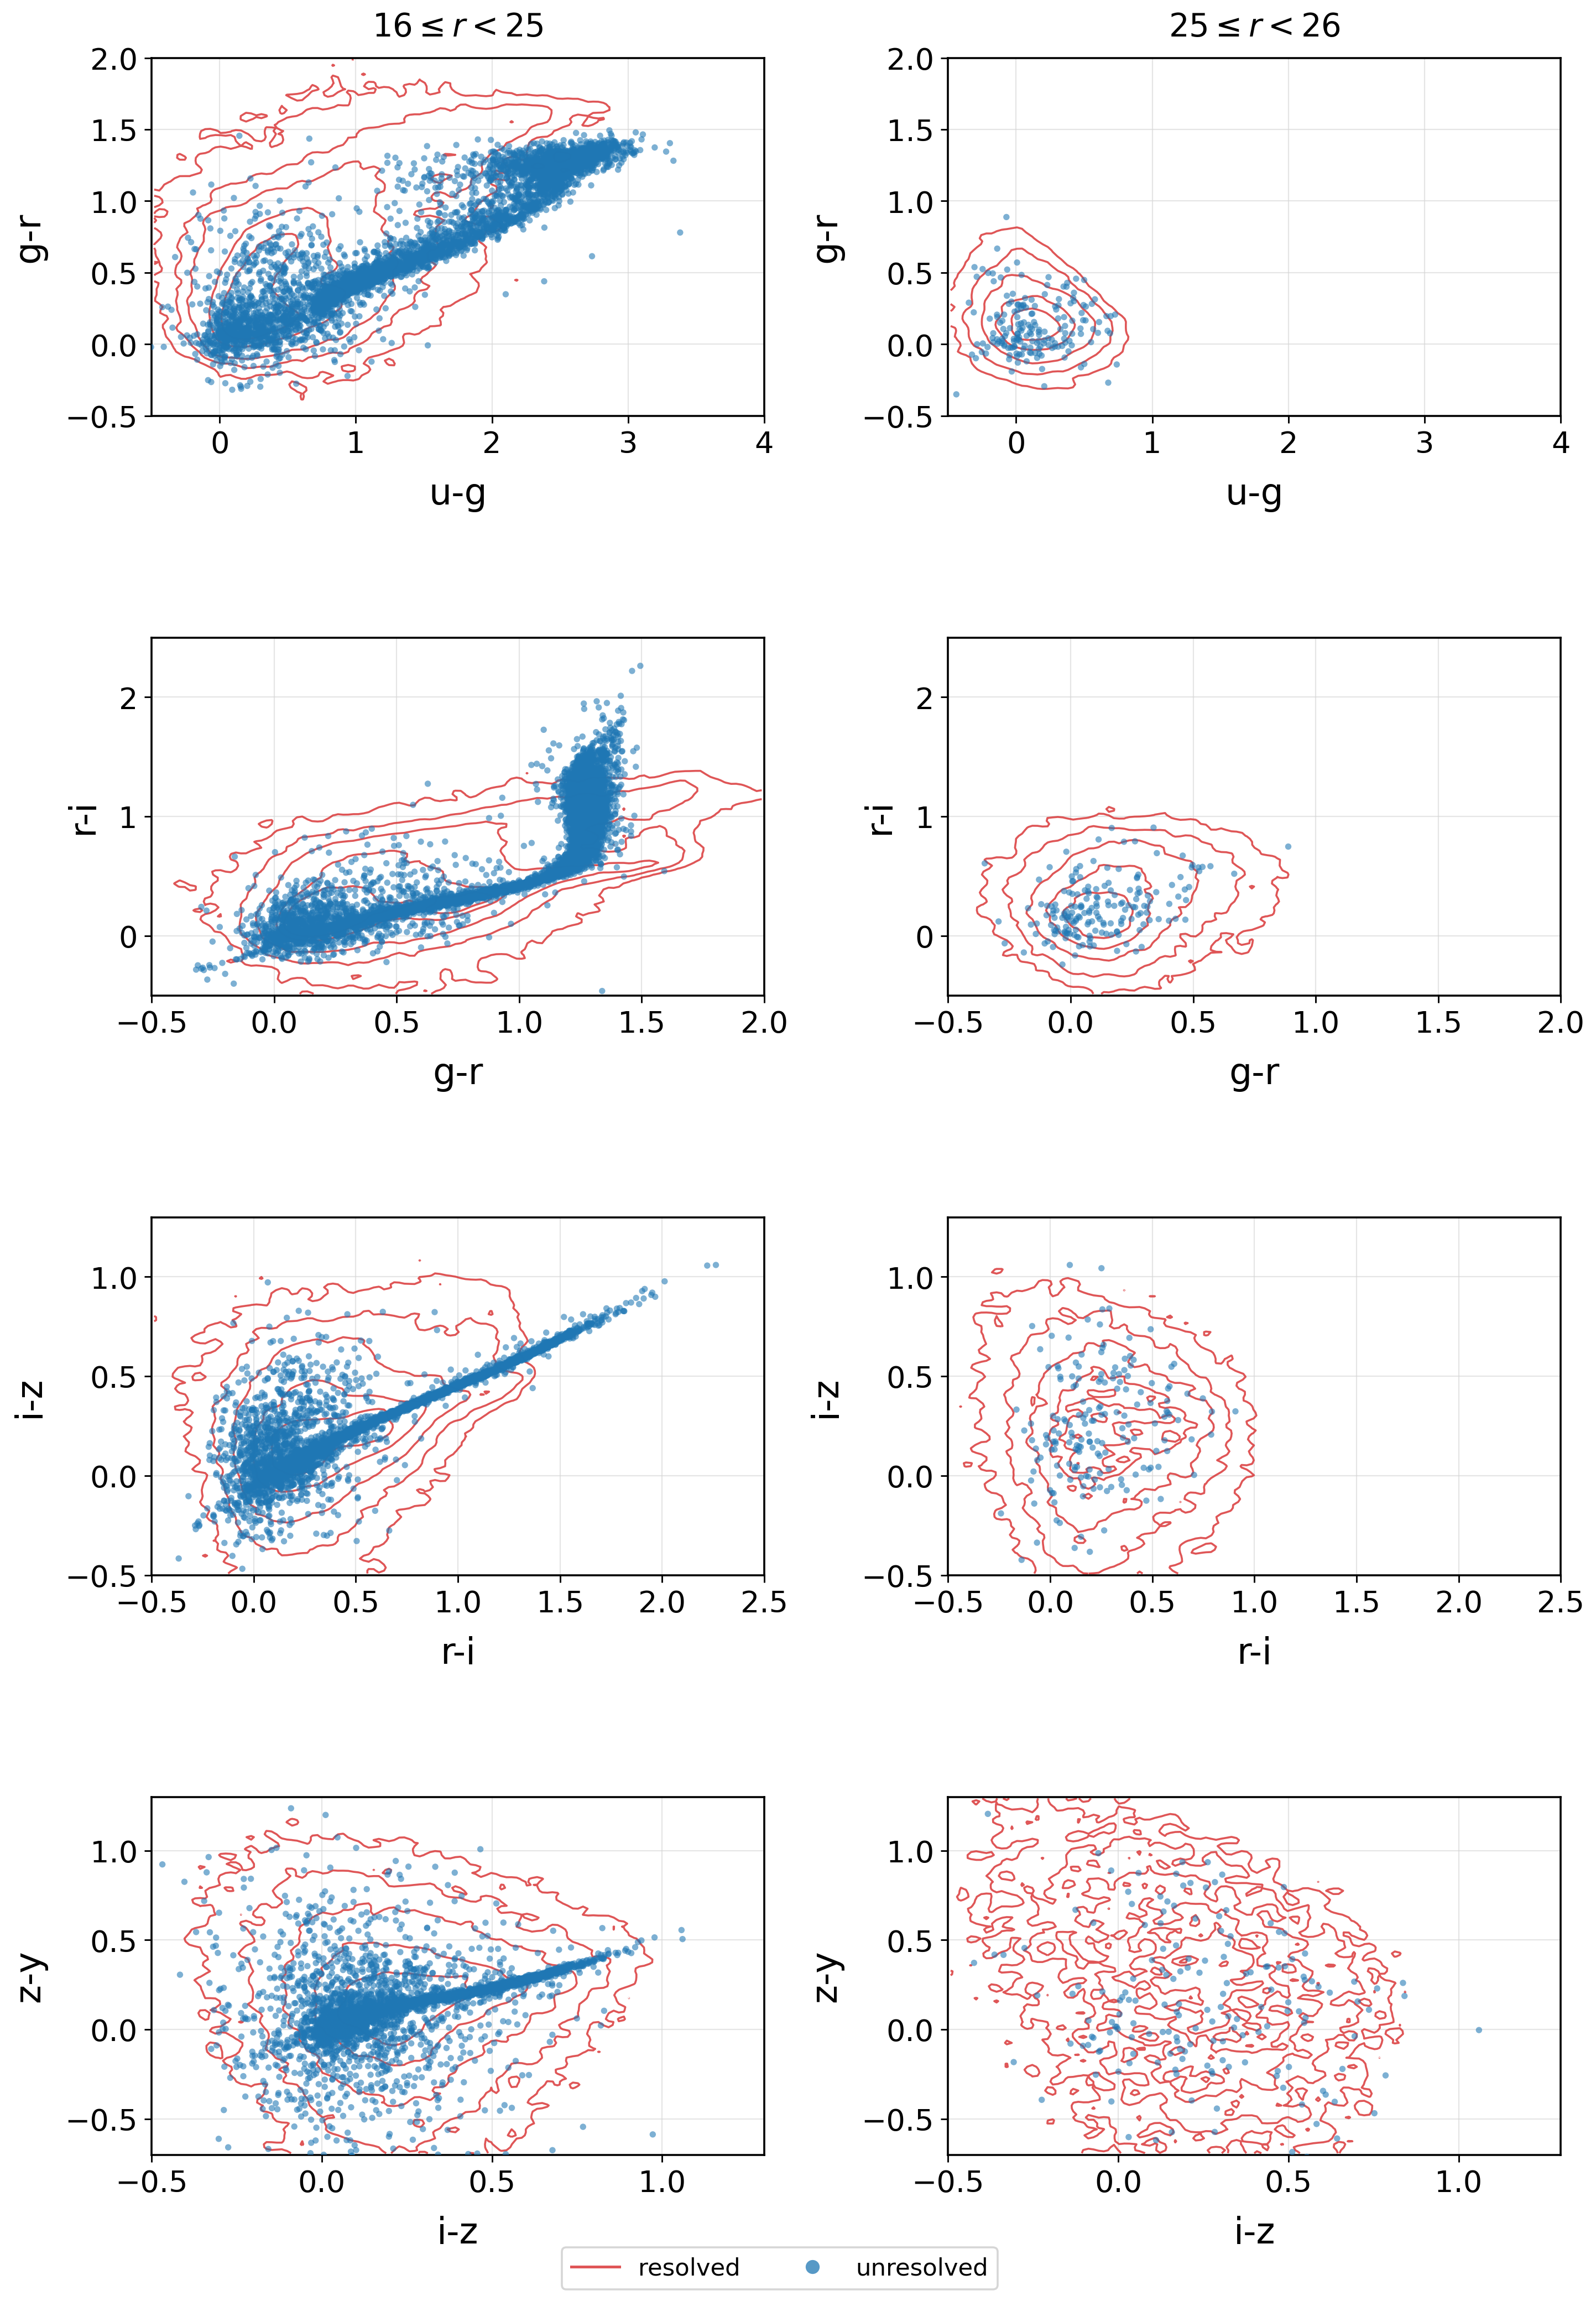
\includegraphics[width=\textwidth,height=0.64\textheight,keepaspectratio]{fig12_ugrizy_color_method_labels.png}
    \caption{Color--color distributions of the samples assigned to the unresolved
    and resolved classes by the combined $ugrizy$ morphology-plus-color
    classifier, shown for $16\leq r<25$ (left) and $25\leq r<26$ (right).  Blue
    points show unresolved assignments, and red contours show the resolved
    population.  The two intervals contain 5,855 and 180 unresolved assignments
    and 106,740 and 25,707 resolved assignments, respectively.  The overlap in
    the individual two-dimensional projections shows that the final assignment
    cannot be represented by a single color--color boundary.}
    \label{fig:color-distributions}
\end{figure*}

Classifier-selected unresolved objects are plotted as blue points, while red
density contours show the classifier-selected resolved population.  The
$16\leq r<25$ interval contains 5,855 unresolved and 106,740 resolved
assignments; the $25\leq r<26$ interval contains 180 and 25,707, respectively.
The small number of faint unresolved assignments accounts for the sparse blue
sample in the right column.  In each individual projection, the blue points
and red contours overlap substantially.  The final classification is
therefore not equivalent to a simple boundary in any one of these
color--color planes; it uses their joint information together with
morphology.

Taken together, the results show that modeling the $r$-band morphology
distributions improves the global AUC relative to raw $\Delta m_r$, although
the ROC curves cross and the gain is not uniform over all false-positive
rates.  At the fixed $p_{{\rm S},r}=0.5$ boundary, the prior-informed $r$-band
selection becomes increasingly conservative and selects no star-like objects
in the faintest interval.  In the multiband comparison, the incremental AUC
gain from color increases toward fainter magnitudes within the evaluated
sample.

\FloatBarrier



- modeling dmag vs. mag using KDE: 2021PASP..133e4502M 

- GP classifier with 5,000 simulated training observations
     averaged over 100 simulation iterations: area under the curve is 0.985
     2022AJ....163..148M 

 

TRACTS vs. PATCHES
LA
In the Rubin Science Pipelines, tracts and patches are the two levels of spatial subdivision used
for coadds and object catalogs. They are designed to make processing and storage scalable
while preserving continuity across the sky. A tract is a relatively large region of the sky,
approximately 1.75$^\deg$ x 1.75$^\deg$ (the exact size depends on the sky map projection).
that is processed as a unit. Tracts overlap slightly with neighboring tracts to avoid edge effects.
Each tract has a unique integer tract ID (e.g., 9813). Tracts are defined by a sky map
(e.g., the RingsSkyMap used for DP1 and DP2).  

Each tract is subdivided into a regular grid of patches, indexed by two integers, with each tract
in DP1/DP2 containing 9 × 9 = 81 patches. The patch size is about 12 arcmin by 12 arcmin
(approximately, one CCD). Patches overlap slightly with neighboring patches. A patch is the basic
processing unit for many pipeline tasks, such as source detection, measurement, and deblending.
This two-level hierarchy offers several advantages.
tracts keep astrometric and photometric calibration consistent over a large area,
define a convenient unit for coadds and catalogs, and simplify distributed processing.
Patches allow parallel processing on many CPUs, keep memory requirements manageable,
and localize expensive tasks such as deblending.



WE MAY NEED IT FOR LATER (Daniel added it, ZI removed it as it was redundant with Introduction:

The principal per-band morphology statistic used throughout this analysis is
\begin{equation*}
    \Delta m_b \equiv  m_{{\rm PSF},b}-m_{{\rm CModel},b}.
\end{equation*}
where $b$ denotes a photometric band.  For an unresolved source, the PSF and CModel measurements agree within
their uncertainties and $\Delta m_b\simeq0$, whereas a resolved source generally has
$\Delta m_b>0$ because the PSF-weighted flux does not capture all of its extended light.


DP2 info:
https://dp2.lsst.io/



ZI notes:
- we need to look at the CMDs representing confusion matrix, as we add more bands
- we need to try Random Forest using HST labels as training set and compare ROC curves with extendeness;
       then also add colors as compare (recycle ZI code for RF that exists somewhere)
- test r_sizeExtendedness, r_model extendedness, griz model extendedness (see Pai et al. 2026)
- when comparing r, gri and ugrizy, the sample must be fixed
- r_extendedness must be be on r-only ROC curve by definition

 

DANIEL:

I just pushed my manuscript edits for this morning (here). I think the first two sections are in
good shape. I will now focus on Section 3. ``Methodology and Performance'' and will complete
the last section once all the plots and analysis are done. I have a few minor things for Daniel
to help me with: 
- Figure 3: please remove the title and overplot unresolved sources with r>24.5 with some other
      color (green?) to distinguish them from bright sources
- please verify that the object counts shown in Figure 5 and reported in Section 2.2 are consistent 
      (by adding numbes in Fig. 5, I get 155,131 but we said 193,586 in Sec 2.2)
- Figure 4: please remove the title and decrease slightly the amount of vertical white space between
         the panel rows (so that figure becomes a bit shorter) 
- can you please find this text in Section 2.5 and add this info?
           DANIEL: can you please add a paragraph here  about how you rejected some HST stars by colors
                         and what were the numbers (fractions) of rejected objects (and how you handled variation 
                         with magnitude? 

      


